\documentclass[a4paper,12pt,twoside,openany]{report}
%
% Wzorzec pracy dyplomowej
% J. Starzynski (jstar@iem.pw.edu.pl) na podstawie pracy dyplomowej
% mgr. inż. Błażeja Wincenciaka
% Wersja 0.1 - 8 października 2016
%
\usepackage{polski}
\usepackage{helvet}
\usepackage[T1]{fontenc}
\usepackage{anyfontsize}
\usepackage[utf8]{inputenc}
\usepackage[pdftex]{graphicx}
\usepackage{tabularx}
\usepackage{array}
\usepackage[polish]{babel}
\usepackage{subfigure}
\usepackage{amsfonts}
\usepackage{verbatim}
\usepackage{indentfirst}
\usepackage[pdftex]{hyperref}


% rozmaite polecenia pomocnicze
% gdzie rysunki?
\newcommand{\ImgPath}{.}

% oznaczenie rzeczy do zrobienia/poprawienia
\newcommand{\TODO}{\textbf{TODO}}


% wyroznienie slow kluczowych
\newcommand{\tech}{\texttt}

% na oprawe (1.0cm - 0.7cm)*2 = 0.6cm
% na oprawe (1.1cm - 0.7cm)*2 = 0.8cm
%  oddsidemargin lewy margines na nieparzystych stronach
% evensidemargin lewy margines na parzystych stronach
\def\oprawa{1.05cm}
\addtolength{\oddsidemargin}{\oprawa}
\addtolength{\evensidemargin}{-\oprawa}

% table span multirows
\usepackage{multirow}
\usepackage{enumitem}	% enumitem.pdf
\setlist{listparindent=\parindent, parsep=\parskip} % potrzebuje enumitem

%%%%%%%%%%%%%%% Dodatkowe Pakiety %%%%%%%%%%%%%%%%%
\usepackage{prmag2017}   % definiuje komendy opieku,nrindeksu, rodzaj pracy, ...


%%%%%%%%%%%%%%% Strona Tytułowa %%%%%%%%%%%%%%%%%
% To trzeba wypelnic swoimi danymi
\title{Implementacja gry “Turbo Slam Dunk Unleashed” z trybem online multiplayer w środowisku Unity}

% autor
\author{Szymon Piórkowski}
\nrindeksu{279065}

\opiekun{dr hab. inż. Paweł Piotrowski}
%\konsultant{prof. Dzielny Konsultant}  % opcjonalnie
\terminwykonania{28 stycznia 2017} % data na oświadczeniu o samodzielności
\rok{2017}


% Podziekowanie - opcjonalne
\podziekowania{\noindent
{\Large Podziękowania}
\bigskip

Dziękujemy bardzo serdecznie wszystkim, a w szczególności Rodzinom i~Unii Europejskiej...

\bigskip

{\raggedleft
Zdolny Student i Pracowity Kolega

}

}

% To sa domyslne wartosci
% - mozna je zmienic, jesli praca jest pisana gdzie indziej niz w ZETiIS
% - mozna je wyrzucic jesli praca jest pisana w ZETiIS
%\miasto{Warszawa}
%\uczelnia{POLITECHNIKA WARSZAWSKA}
%\wydzial{WYDZIAŁ ELEKTRYCZNY}
\instytut{INSTYTUT ELEKTROENERGETYKI}
\zaklad{ZAKŁAD SIECI I SYSTEMÓW ELEKTROENERGETYCZNYCH}
%\kierunekstudiow{INFORMATYKA}

% domyslnie praca jest inzynierska, ale po odkomentowaniu ponizszej linii zrobi sie magisterska
%\pracamagisterska
%%% koniec od P.W

\opinie{%
  \newpage
\begin{center}
 {\large\bf  Opinia} \\
o pracy dyplomowej magisterskiej wykonanej przez dyplomanta\\
{\bf Zdolnego Studenta i Pracowitego Kolegę} \\
 Wydział Elektryczny, kierunek Informatyka,  Politechnika Warszawska\\
Temat pracy\\
\textit{\bf
TYTUŁ PRACY DYPLOMOWEJ
}\\
\end{center}
\medskip
\noindent
Promotor: {\bf dr inż. Miły Opiekun}\\
Ocena pracy dyplomowej: {\bf bardzo dobry}

\medskip

\centerline{\bf Treść opinii}
   Celem pracy dyplomowej panów dolnego Studenta i Pracowitego Kolegi  było
opracowanie systemu pozwalającego symulować  i opartego o oprogramowanie o
otwartych źródłach (ang. Open Source). Jak piszą Dyplomanci, starali się opracować
system, który łatwo będzie dostosować do zmieniających się dynamicznie wymagań,
będzie miał niewielkie wymagania sprzętowe i umożliwiał dalszą łatwą rozbudowę oraz
dostosowanie go do potrzeb.
Przedstawiona do recenzji praca składa się z krótkiego wstępu jasno i
wyczerpująco opisującego oraz uzasadniającego cel pracy, trzech rozdziałów (2-4)
zawierających opis istniejących podobnych
rozwiązań, komponentów rozpatrywanychjako kandydaci do
tworzonego systemu i wreszcie zagadnień wydajności wirtualnych
rozwiązań. Piąty rozdział to opis przygotowanego przez
Dyplomantów środowiska obejmujący opis konfiguracji
środowiska oraz przykładowe ćwiczenia laboratoryjne. Ostatni
rozdział pracy to opis możliwości dalszego
rozwoju projektu. W ramach przygotowania pracy Dyplomanci zebrali i przedstawili w
bardzo przejrzysty sposób duży zasób informacji, co świadczy o dobrej orientacji
w nowoczesnej i ciągle intensywnie rozwijanej tematyce stanowiącej
zakres pracy i o umiejętności przejrzystego przedstawienia tych
wyników. Praca zawiera dwa dodatki, z których pierwszy obejmuje wyniki
eksperymentów i badań nad wydajnością, a drugi to źródła
skryptów budujących środowisko.

 Dyplomanci dość
dobrze zrealizowali postawione przed nimi zadanie,
wykazali się więc umiejętnością zastosowania w praktyce wiedzy
przedstawionej w rozdziałach 2-4.  Uważam, że cele postawione w założeniach pracy zostały pomyślnie
zrealizowane. Proponuję ocenę bardzo dobrą (5).

\vskip 1cm
{
\raggedleft
(data, podpis)\kern1cm

}
  \newpage
  \newpage
\begin{center}
 {\large\bf  Recenzja } \\
pracy dyplomowej magisterskiej wykonanej przez dyplomanta\\
{\bf Zdolnego Studenta i Pracowitego Kolegę} \\
 Wydział Elektryczny, kierunek Informatyka,  Politechnika Warszawska\\
Temat pracy\\
\textit{\bf
TYTUŁ PRACY DYPLOMOWEJ
}\\
\end{center}
\medskip
\noindent
Recenzent: {\bf prof. nzw. dr hab. inż. Jan Surowy}\\
Ocena pracy dyplomowej: {\bf bardzo dobry}
\medskip


\centerline{\bf Treść recenzji}
   Celem pracy dyplomowej panów dolnego Studenta i Pracowitego Kolegi  było
opracowanie systemu pozwalającego symulować  i opartego o oprogramowanie o
otwartych źródłach (ang. Open Source). Jak piszą Dyplomanci, starali się opracować
system, który łatwo będzie dostosować do zmieniających się dynamicznie wymagań,
będzie miał niewielkie wymagania sprzętowe i umożliwiał dalszą łatwą rozbudowę oraz
dostosowanie go do potrzeb.
Przedstawiona do recenzji praca składa się z krótkiego wstępu jasno i
wyczerpująco opisującego oraz uzasadniającego cel pracy, trzech rozdziałów (2-4)
zawierających bardzo solidny i przejrzysty opis: istniejących podobnych
rozwiązań (rozdz. 2), komponentów rozpatrywanychjako kandydaci do
tworzonego systemu (rozdz. 3) i wreszcie zagadnień wydajności wirtualnych
rozwiązań, zwłaszcza w kontekście współpracy  kilku elementów
 sieci (rozdział 4). Piąty rozdział to opis przygotowanego przez
Dyplomantów środowiska obejmujący opis konfiguracji
środowiska oraz przykładowe ćwiczenia laboratoryjne (5 ćwiczeń). Ostatni, szósty
rozdział pracy to krótkie zakończenie, które wylicza także możliwości dalszego
rozwoju projektu. W ramach przygotowania pracy Dyplomanci zebrali i przedstawili w
bardzo przejrzysty sposób duży zasób informacji o narzędziach, Rozdziały 2, 3 i 4 świadczą o dobrej orientacji
w nowoczesnej i ciągle intensywnie rozwijanej tematyce stanowiącej
zakres pracy i o umiejętności syntetycznego, przejrzystego przedstawienia tych
wyników. Drobne  mankamenty tej części pracy to zbyt skrótowe omawianie
niektórych zagadnień technicznych, zakładające dużą początkową wiedzę czytelnika
i dość niestaranne podejście do powołań na źródła.
Utrudnia to w pewnym stopniu czytanie pracy i zmniejsza jej wartość dydaktyczną
(a ta zdaje się być jednym z celów Autorów), ale jest zrekompensowane zawartością
merytoryczną. Praca zawiera dwa dodatki, z których pierwszy obejmuje wyniki
eksperymentów i badań nad wydajnością, a drugi to źródła
skryptów budujących środowisko. Praca
zawiera niestety dość dużą liczbę drobnych błędów redakcyjnych, ale nie wpływają
one w sposób istotny na na jej czytelność i wartość. W całej pracy przewijają
się samodzielne, zdecydowane wnioski Autorów, które są wynikiem własnych i
oryginalnych badań.  Rozdział 5 i dodatki pracy przekonują mnie, że Dyplomanci dość
dobrze zrealizowali postawione przed nimi zadanie. Pozwala to stwierdzić, że
wykazali się więc także umiejętnością zastosowania w praktyce wiedzy
przedstawionej w rozdziałach 2-4. Kończący pracę rozdział szósty świadczy o
dużym (ale moim zdaniem uzasadnionym) poczuciu własnej wartości i jest
świadectwem własnego, oryginalnego spojrzenia na tematykę przedstawioną w pracy
dyplomowej. Uważam, że cele postawione w założeniach pracy zostały pomyślnie
zrealizowane. Proponuję ocenę bardzo dobrą (5).

\vskip 1cm
{
\raggedleft
(data, podpis)\kern1cm

}
}

\streszczenia{
  \newpage
\begin{center}
\large \bf
Implementacja gry ,,Turbo Slam Dunk Unleashed'' z trybem online multiplayer w środowisku Unity
\end{center}

\section*{Streszczenie}
W ramach pracy dyplomowej zaimplementowano grę komputerową Turbo Slam Dunk Unleashed w środowisku Unity. Projekt został wykonany w języku C\#. Gra została pierwotnie stworzona w środowisku Game Maker Studio, w 2016 roku.
Gra została napisana od początkowi w nowej technologi w celu polepszenia jej jakości oraz zwiększenia możliwości dodawania nowych funkcjonalności. Ponadto została ona rozszerzona o moduł multiplayer, a także wstępnie przygotowana do przeniesienia na nowe platformy (Linux, konsole do gier).

\bigskip
{\noindent\bf Słowa kluczowe:} Unity, C\#, gra komputerowa, grafika komputerowa, Game Maker Studio

\vskip 2cm



\newpage
\begin{center}
\large \bf
Implementation of the game ``Turbo Slam Dunk Unleashed'' in Unity platform, including online multiplayer mode 
\end{center}

\section*{Abstract}
As a part of the diploma thesis, the game Turbo Slam Dunk Unleashed has been implemented in Unity enviroment The proejct has been made using the C\# language. The Game was orginally created in Game Maker Studio enviroment in 2016. Moreover, the game has been extended by online multiplayer module, and pre-prepared to be deployed to new platforms (Linux, game consoles)

\bigskip
{\noindent\bf Keywords:} Unity, C\#, computer game, computer graphics, Game Maker Studio

\vfill
}

\begin{document}
\maketitle

%-----------------
% Wstęp
%-----------------
\chapter{Wstęp}
Celem niniejszej pracy jest przeniesienie gry Turbo Slam Dunk Unleashed do środowiska Unity oraz dodanie do niej modułu online multiplayer. Ponadto, podjęte zostały kroki w celu ułatwienia przygotowania projektu do uruchomienia na nowych platformach. W tym celu gra musiała zostać napisana od zera w języku C\#. Pierwotnie gra została stworzona przez autora niniejszej pracy w środowisku Game Maker.

\section{Gry Komputerowe}
Gry Komputerowe to zagadnienie które początków można szukać już nawet przed stworzeniem pierwszych komputerów osobistych z wyświetlaczami. Mało osób wie, że pierwsze gry były produkcjami akademickimi. Takie gry technicznie nie różnią się bardzo od innych programów komputerowych. Kluczową różnicą jest cel ich powstania. Głównym celem gier jest dostarczenie użytkownikowi rozrywki.

W dzisiejszych czasach gry są już niemal wszędzie. Mimo tak krótkiej historii istnieją już klasyki które zna znakomita większość graczy. Zdecydowana większość osób młodych miała z już nimi styczność. Popularność gier można zawdzięczać chociażby faktowi, że gry powstają na niemalże każdą platformę elektroniczną - od starszych telefonów komórkowych z dedykowanymi systemami operacyjnymi po nowoczesne konsole do gier. Do ciekawszych przykładów platform na które stworzone zostały gry można zaliczyć: oscyloskopy, czytniki ebooków, zegarki czy telewizory typu SmartTV. Zjawisko to może być porównane do innych dziedzin kultury.

Sam problem stworzenia gry komputerowej może wydawać się pozornie prosty, ze strony jej odbiorcy, jednak są to jedne z najbardziej zaawansowanych dzieł ludzkich. Poza kompleksowymi problemami natury programistycznej czy algorytmicznej, dobra gra musi przyciągać uwagę użytkownika i zaspokajać jego ciekawość oraz potrzeby rozrywki. Do osiągnięcia tych celów nie rzadko korzysta się z bardzo wielu dziedzin nauki takich jak psychologia, fizyka lub biologia.

Ponadto branża gier komputerowych nie różni się bardzo od branży filmowej czy muzycznej. Powoli zaczyna doganiać ich rozmiar w niektórych krajach, a globalny rynek gier komputerowych przwyższył swoją wartością przemysł filmowy już w 2013 roku. W Polsce z roku na rok branża rośnie i można powiedzieć że polskie gry są jednym z lepszych towarów eksportowych\cite{canalplus_gry}. Zdecydowanie mają przed sobą ciekawą przyszłość. Dlatego też zagadnienie to jest głównym tematem tej pracy. 

\section{Motywacja}
Pierwotnie Gra Turbo Slam Dunk Unleashed została wykonana w środowisku Game Maker Studio. Dawało to wystarczające możliwości jak na prostotę gry, jednak narzucało również dużo ograniczeń oraz komplikacji. Game Maker jest prostym narzędziem do tworzenia gier dwuwymiarowych. Struktura projektu którą narzuca te środowisko sprawia że projekt strasznie trudno się skaluje. Korzysta on z języka skryptowego Game Maker Language (GML) który składa się na skrypty w grze. Z tego powodu pisanie warstwy sieciowej wprowadziłoby chaos w wystarczająco skomplikowanym już projekcie. Ponadto wsparcie dla konsol, mimo swojego istnienia, jest znacznie ograniczone w stosunku do tego w Unity.

Środowisko Unity pozwala pokonać wszystkie te problemy, dodając przy tym projektowi nowego potencjału dla rozwiązywania niektórych, zarówno algorytmicznych jak i designowych problemów w grze. Wsparcie samych twórców silnika jest stabilniejsze w przypadku Unity z prostego powodu - komercyjnych gier tworzonych za jego pomocą jest znacznie więcej. Najważniejszym powodem przepisania gry nie była sama technologia, co postęp doświadczenia twórcy. Finalna wersja gry powstała w 2016 roku. Po 3 latach umiejętności autora znacznie się poprawiły i projekt może zdecydowanie na tym skorzystać. 

\section{Założenia}
Gry komputerowe nie mają jasno określonej granicy skończenia. Zawsze można coś poprawić, dodać czy zmienić. W takim projekcie ważne jest żeby wyznaczyć jasne cele i wymagania które doprowadzą do stworzenia skończonego produktu. Dlatego też zostały stworzone założenia, które musi spełniać gra żeby uznać ją za kompletną:

\begin{itemize}
    \item Przeniesienie gry w wersji podstawowej do środowiska Unity
    \begin{itemize}
        \item Mecz 2 graczy na 1 komputerze
        \item Rzucanie i zabieranie piłki, faule
        \item Liczenie punktów, stan meczu
        \item Wybór postaci, piłki, planszy oraz czasu meczu
    \end{itemize}
    
    \item Dodanie trybu online multiplayer
    \begin{itemize}
        \item Mecz 2 graczy na 2 komputerach przez sieć
        \item Synchronizacja pozycji graczy oraz piłki
        \item Synchronizacja stanu meczu - punkty, faule, czas i inne
        \item Synchronizacja wyboru ustawień meczu - wygląd graczy, piłki, mapa oraz czas meczu
        \item Możliwość dołączenia do losowego gracza lub gry ze znajomym
        \item obsługa błędów związana z problemami z połączeniem.
    \end{itemize}
    
    \item Przygotowanie gry do przeniesienia na nowe platformy
    \begin{itemize}
        \item Przygotowanie warstwy abstrakcji wejść
        \item Optymalizacja logiki i warstwy sieciowej
    \end{itemize}
\end{itemize}



%-----------------
% Opis Środowiska
%-----------------
\chapter{Opis Środowiska}
W tym rozdziale znajduje się opis narzędzi przy pomocy których został zrealizowany projekt gry.
\section{Unity}
Unity jest częściowo darmowym silnikiem do tworzenia gier stworzonym w 2005 roku. Od tego czasu silnik był wielokrotnie modyfikowany i zostało opublikowane wiele nowych wersji. Obecnie najnowsza stabilna wersja oznaczona jest numerem 2018.3\cite{unity_wiki}. Silnikiem do gry nazywamy zestaw narzędzi, oraz sprawdzonych algorytmów które często używane są do tworzenia gier. Pierwsza wersja Unity została stworzona przez 3 kolegów - Davida Helgason, Joachima Ante oraz Nicholasa Francisa w Dani. Unity posiada kilka typów licencji, podstawowa jest darmowa jednak po przekroczeniu określonego przez Unity półapu przychodów, należy kupić licencję wyższego poziomu. Płatne licencje nie dają tylko takiej możliwości, rozszerzają one nieco możliwości edytora a także zwiększają wsparcie developerów. W przypadku najdroższej wersji - Enterprise, użytkownicy silnika mają nawet dostęp do kodu źródłowego silnika.

\begin{table}[h!]
\centering
\begin{tabular}{c|cccc}
Nazwa Wersji & Limit przychodów & Wsparcie premium & Cena \\ \hline
Personal & \$100,000 & NIE & Darmowa \\
Plus & \$200,000 & NIE & \$420 rocznie \\
Pro & Nielimitowane & TAK & \$1500 rocznie \\
Enterprise & Nielimitowane & TAK & Indywidualnie \\
\end{tabular}
\caption{Zestawienie licencji Unity}
\label{table_unity_versions}
\end{table}

\begin{figure}[!htbp]
	\begin{center}
\centering
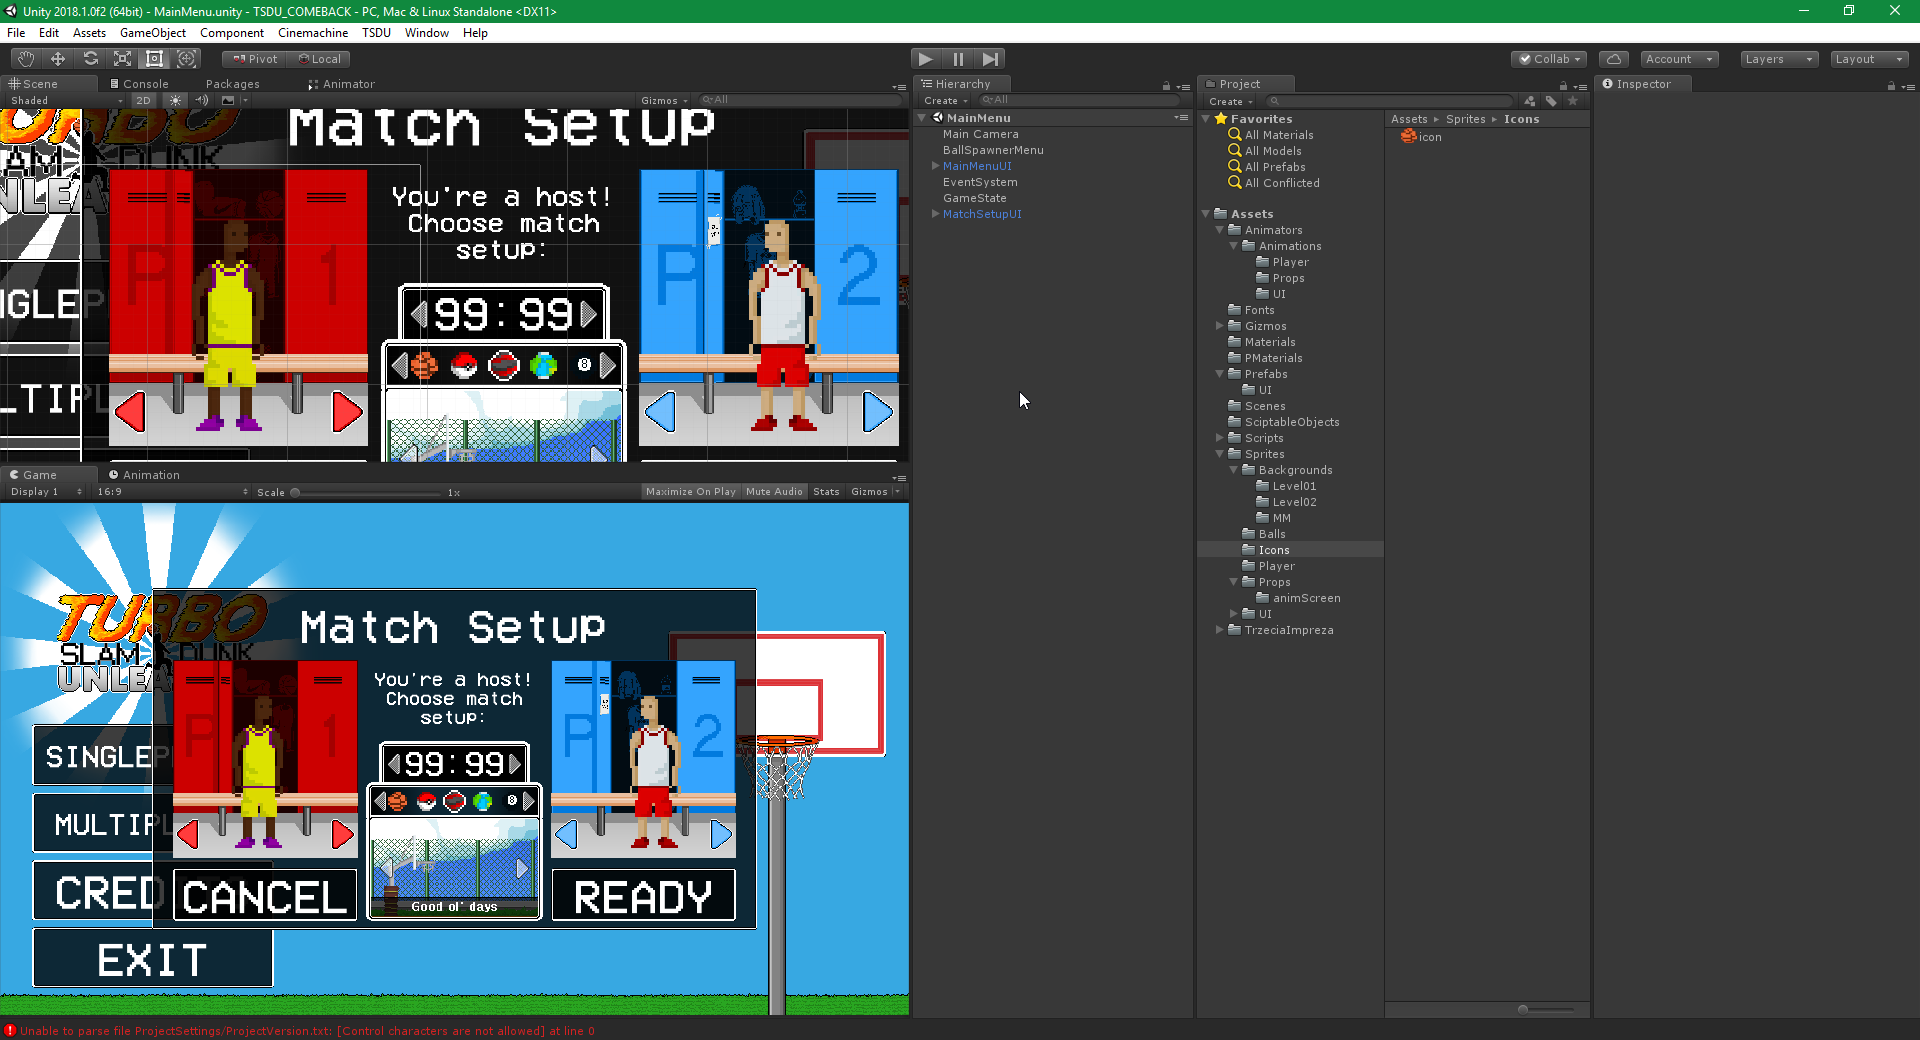
\includegraphics[scale=0.2]{\ImgPath/rys/unity_home.png}
\end{center}
	\caption{Domyślny widok edytora Unity w projekcie gry}
	\label{unity_home}
\end{figure}

Na chwilę obecną silnik obsługuje 27 platform: iOS, Android, Tizen, Windows, Universal Windows Platform, macOS, Linux, WebGL, PlayStation 4, PlayStation Vita, Xbox One, Wii U, 3DS, Oculus Rift, Google Cardboard, SteamVR, PlayStation VR, Gear VR, Windows Mixed Reality, Daydream, Android TV, Samsung Smart TV, tvOS, Nintendo Switch, Fire OS, Facebook Gameroom, Apple's ARKit, Google's ARCore, and Vuforia. Jest to dość długa lista jak na silnik do tworzenia gier. Zwykle ograniczają się one do mniejszej liczby platform. Dlatego też gra stworzona w tym silniku ma bardzo duży potencjał do zaistnienia na większej ilości platform a co za tym idzie - zyskanie nowych graczy. Samo przenisienie między platformą jest reklamowane przez Unity jako bardzo prosta akcja - wystarczy jeden przycisk. W praktyce jednak zależy to bardzo od typu gry oraz tego jak wygląda architektura samej gry.

Sam silnik napisany jest w językach C, C++ oraz C\#. W pierwszych dwóch napisane są podstawy silnika takie jak renderowanie, logika czy obsługa wejść. Trzeci z tych języków został użyty do napisania warstwy wizualnej - GUI edytora oraz do stworzenia podstawowych komponentów. Może on być równiwerz używany przez twórców gier do tworzenia własnych komponentów lub rozszerzeń silnika. Unity przyjmuje podejście komponentowe. Typ obiektu w grze definiuje zestaw jego komponentów. Komponenty są mniejszymi elementami które realizują określone zdania. Do podstawowych typów komponentów można zaliczyć miedzy innymi:
\begin{itemize}
    \item \textit{Transform} - Posiada go każdy GameObject, służy do określenia pozycji, rotacji oraz skali obiektu w przestrzeni trójwymiarowej sceny. Transformy tworzą hierarchie sceny podobną do drzewa. Dzięki temu możemy np. tworzyć skompilowane obiekty na scenie a następnie poruszać je całe poprzez transalcje jednego, nadrzędnego transforma.
    \item \textit{Camera} - Podstawa renderingu, wyświetla na danym ekranie część sceny na którą aktualnie obejmuje. Posiada 2 tryby projekcji - ortogonalną oraz perspektywiczną. Z zasady pierwszy typ wykorzystywany jest dla gier dwuwymiarowych natomiast drugi dla trójwymiarowych.
    \item \textit{Sprite Renderer} - Komponent odpowiedzialny za rysowanie dwuwymiarowych obrazków - tzw. Spritów. Posiada różne tryby rysowania, obroty w osiach X i Y, kolejność sortowania oraz możliwość przemnożenia kolorów obrazka przez jeden wybrany kolor,
    \item \textit{Box Collider 2D} - Komponent ten umożliwia rejestrowanie kolizji - fundamentalnej funkcjonalności gry. Kolizje występują kiedy dwa obiekty są w kontakcie, a także dostarczają szczegółowych informacji o tych kontaktach. Typ Box jest prostszym kształtem, istnieją też inne bardziej lub mniej skomplikowane kształty colliderów.
    \item \textit{Rigidbody 2D} - Podstawa symulacji fizyki dwuwymiarowej w Unity. Obiekt posiadający ten komponent musi również posiadać komponent typu Collider 2D żeby móc odbierać informacje o kolizjach. Posiada zestaw zmiennych umożliwiających symulację fizyki: masa, pozycja, prędkość, prędkość kątowa oraz środek ciężkości. Ulega też grawitacji jeżeli taka jest zdefiniowana na scenie.
    \item \textit{Animator} - Odpowiada za animacje niemalże dowolnej wartości obiektu. Poprzez animacje możemy rozumieć zmianę wartości w czasie. Najczęściej służy do zmiany pozycji obiektów, ale można nim także zmieniać pojedyncze zmienne komponentów takie jak kolor czy sprite. Animator jest realizowany w postaci maszyny stanów.
    \item \textit{Canvas} - Podstawa interfejsu użytkownika. Definiuje przestrzeń w której wyświetlane są jego elementy. Może być ona wyświetlana jako narzuta na okno gry, narzuta na konkretną kamerę, lub płaszczyzna w przestrzeni trójwymiarowej.
    \item \textit{Mono Behavior} - Komponenty tego typu są skryptami w języku C\#. Można więc swobodnie je definiować i stworzyć w nich niemalże dowolną funkcjonalność. Więcej informacji o skryptowaniu znajduje się w sekcji "Język C\# oraz Mono"
\end{itemize}
Powyższe elementy są najczęściej wykorzystywane podczas tworzenia gry dwuwymiarowej. Istnieje szereg komponentów o funkcjonalności trójwymiarowej, ale jako że gra opisywana w tej pracy operuje tylko na dwóch wymiarach zostały one pominięte.

\section{Język C\# oraz Mono}

Do programowania rozgrywki oraz logiki gry używa się języka C\#. Nie jest on jednak natywnym językiem silnika. Żeby możliwe było obsługiwanie Skryptów w tym języku Unity używa zewnętrznej platformy zwaną Mono. Mono jest open-sourcowym projektem opartym na frameworku .Net\cite{about_mono}. Pozwala między innymi na łatwe budowanie aplikacji na wiele platform.

\begin{figure}[!htbp]
	\begin{center}
\centering
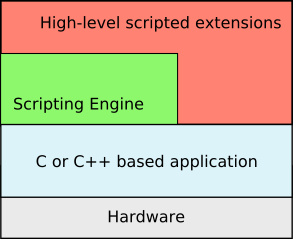
\includegraphics[scale=0.6]{\ImgPath/rys/mono_architecture_scripting.png}
\end{center}
	\caption{Architektura implementacji C\# jako język skryptowy w Mono}
	\label{mono_architecture_scripting}
\end{figure}

W przeszłości do podobnych celów wykorzystywało się języki skryptowe. Wiele silników posiadało własne mniej lub bardziej wydajne implementacje. Często jednak wielkość skryptów przekraczała możliwości interpretatora lub nawet silnika skryptowania przez co możliwości były bardzo ograniczone. Mono używa różnych języków do różnych celów, a więc traktuje je jako narzędzia które służą do rozwiązywania innych problemów.

Podczas gdy ważna, krytyczna część aplikacji może być napisana w wydajnym nisko poziomowym języku jak C, częściami takimi jak interfejs użytkownika czy interakcje z użytkownikiem zajmuje się język wyższego poziomu który nie jest tak samo wydajny ale pozwala zmniejszyć ilość wymaganych linijek kodu do zrealizowania konkretnego zadania. Kod napisany w takim języku jest zdecydowanie wolniejszy od kodu natywnego ale w porównaniu z popularnymi językami skryptowymi takimi jak np. LUA jest zdecydowanie szybszy. Mono umożliwia bardzo proste wołanie metod w języku natywnym przez co łatwo jest podzielić zadania na te które powinny być napisane optymalnie, a te które nie wymagają aż takiej oszczędności. Wspierane jest wiele języków wyższego poziomu do których należą miedzy innymi: C\#, Java, F\#, Python czy JavaScript.

Język C\# jest stworzonym dla Microsoft obiektowym językiem programowania. Kod napisany w tym języku kompilowany jest do Common Intermediate Language (CIL) który jest z kolei wykonywany w środowisku uruchomieniowym  takim jak .Net czy właśnie Mono.  


\begin{figure}[!htbp]
	\begin{center}
\centering
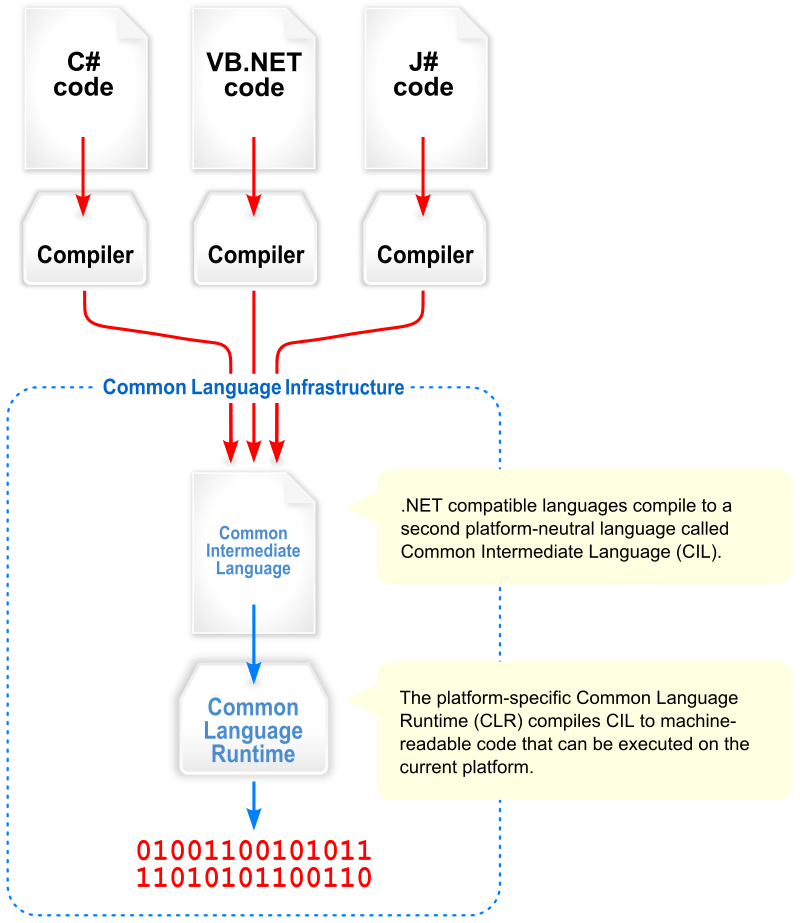
\includegraphics[scale=0.43]{\ImgPath/rys/CIL.png}
\end{center}
	\caption{Schemat pokazujący proces kompilacji języka wykorzystującego CIL}
	\label{CIL}
\end{figure}

Język ten jest silnie typowany, deklaratywnym imperatywny oraz funkcyjny. Powstał w około 2000 roku i został zaakceptowany jako standard przez ECMA (ECMA-334) oraz ISO (ISO/IEC 23270:2006). Posiada wiele przydatnych funkcji:
\begin{itemize}
    \item Odśmiecanie pamięci - C\# automatyczne zarządzą pamięcią poprzez liczenie referencji do obiektów. Jeżeli do danego obiektu nie prowadzi żadna referencja jest on niszczony podczas przebiegu tzw Garbage collectora
    \item Delegaty oraz Zdarzenia - bardzo wygodny sposób na kontrolowanie wykonywania kodu i uruchomienie go podczas zdarzeń. Jest to pewnym rozszerzeniem wskaźników które możemy spotkać w językach niższego poziomu.
    \item Refleksja i atrybuty klas - Podczas działania programu istnieje możliwość analizy jego struktury z poziomu tego kodu. Przydaje się chociażby podczas debugowania kodu czy innych zastosowaniach które korzystają z nieznanej podczas kompilacji struktury kodu.
    \item Typy generyczne - mechanizm zbliżony do działania szablonów w C++. Pozwala na tworzenie całych klas operujących na danych o nieznanym typie ale posiadającym konkretny zestaw funkcji.
\end{itemize}

\section{Dodatkowe narzędzia}
Do stworzenia kompletnej gry teoretycznie wystarczy sam silnik jednak używnie zewnętrznych programów do tworzenia plików znacznie poprawia jakość zarówno samej produkcji jak i pracy nad nią. Poniżej znajduje się listą użytego oprogramowania:

\begin{itemize}
    \item Microsoft Visual Studio 2017 - środowisko programistyczne wspierające wiele języków. Możliwe jest doinstalowanie pakietu integracji z Unity. Poza edycją skryptów pozwala na debugowanie projektu poprzez wbudowany debugger.
    \item Git - Darmowy i open sourcowy program służący do kontroli wersji.Jest to program konsolowy. Bardzo przydaje się do śledzenia zmian, a także do łatwego tworzenia kopi zapasowej plików projektowych.
    \item Git Extensions - Darmowy i open sourcowy program do obsługi gita. Uzupełnia gita o graficzny interfejs co ułatwia pracę przy dużych projektach. Zamyka też wiele skomplikowanych komend w przystępne guziki co uprzyjemnia pracę z gitem.
    \item Paint.Net - Darmowy i open sourcowy program do edycji grafiki. Napisany w języku C\# z wykorzystaniem frameworku .Net. Bardzo prosty w obsłudze program dzięki któremu poprawki grafiki zostały wykonane szybko i precyzyjnie bez utraty jakości.
    \item TexturePacker - Program do pakowania obrazków w tzw. atlasy. Taki sposób przechowywania obrazków umożliwia prostsze animowanie, jest wydajniejszy pamięciowo oraz pozwala ominąć kilka innych problemów związanych z importowaniem dużej ilości obrazków do projektu z grą.
\end{itemize}

%-----------------
% Opis gry “Turbo Slam Dunk Unleashed”
%-----------------
\chapter{Opis gry “Turbo Slam Dunk Unleashed”}

\section{Historia}

Proces tworzenia gry rozpoczął się w 2015 roku, a jej pełna wersja została udostępniona w serwisie Gamejolt.com 3 czerwca 2016 roku\cite{gamejolt_page}. Na początku był to projekt hobbystyczny, który potem zamienił się w projekt kołowy i był tworzony w ramach Koła Naukowego Twórców Gier "Polygon". Finalna wersja została zaprezentowana na jednym z pokazów projektów kołowych.
\begin{figure}[!htbp]
	\begin{center}
\centering
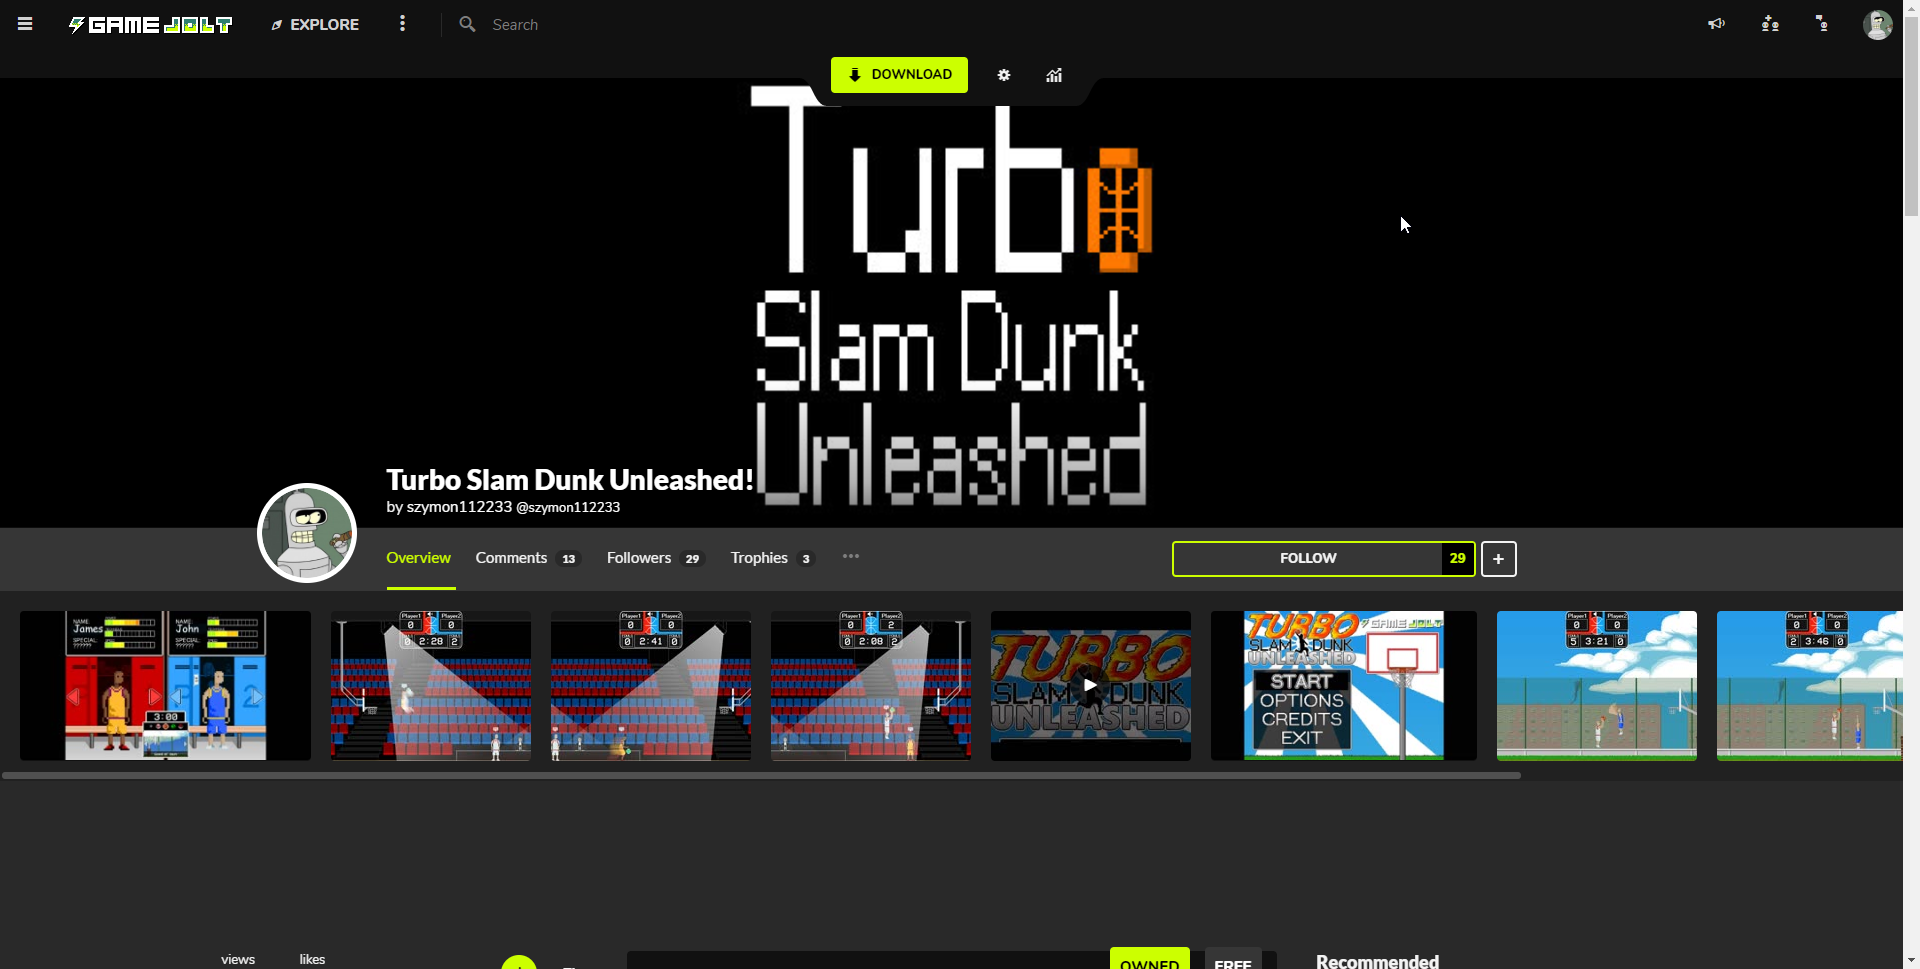
\includegraphics[scale=0.25]{\ImgPath/rys/gamejolt_page.png}
\end{center}
	\caption{Strona główna gry w serwise Gamejolt.com}
	\label{gamejolt_page}
\end{figure}

\section{Ogólny opis gry}
Głównym elementem rozgrywki są mecze koszykówki miedzy dwoma graczami rywalizującymi na jednym komputerze. Gracze używają jednej klawiatury lub padów żeby poruszać swoimi postaciami w świecie gry. Istnieje jedna piłka, której wrzucenie do kosza przeciwnika powoduje zdobycie punktu. W grze istnieją również faule. Faul to sytuacja gdy jeden gracz uderzy drugiego żeby zabrać mu piłkę  w które gracz wyskoczył z piłką i jej nie rzucił - tak jak w prawdziwej koszykówce. Faule są liczone i odejmowane od zdobytych punktów pod koniec meczu. Mecz trwa określony czas, domyślenie 3 minuty i po tym czasie liczone są punkty i wyświetlany jest werdykt meczu.

\section{Opis elementów gry}

Gra jest bardzo prosta i składa się z kilku podstawowych elementów.
Poniżej znajduje się obrazek pokazujacy graficzne reprezantacje wymienionych elementów.
\begin{enumerate}
    \item Plansza - Świat gry w którym poruszają się gracze, głównie są to elementy wizualne
    \item Postacie graczy - W grze istnieją 2 instancje. Jest ona sterowana przez człowiek poprzez zestaw wejść. Może chodzić w lewo lub w prawo, skakać, rzucać piłkę oraz uderzać. Dwie ostatnie akcje możliwe są zarówno podczas stania jak i w locie. Skok służy do zwiększenia zasięgu rzutu lub po prostu lepszego do niego ustawienia. Obrót gracza jest niemożliwy w powietrzu, pozwala to na dokładniejsze dostosowanie swojej pozycji do rzutu. Rzut piłki służy głownie do umiejscowienia jej w obręczy kosza. Po rozpoczęciu przyciskania klawisza odpowiedzialnego za rzut, gracz traci możliwość chodzenia i jest w trakcie rzutu. Podczas tego czasu pokazuje się wskaźnik siły rzutu który oscyluje między minimalną i maksymalna siłą rzutu. Po puszczeniu przycisku piłka jest rzucana zgodnie z siłą która była wskazana w tym momencie. Uderzanie służy do zabierania piłki drugiemu graczowi. Po przyciśnięciu klawisza uderzenia rozpoczyna się animacja uderzenia i jeżeli trafiliśmy ręką w punkt w którym znajduje się piłka piłka jest wybijana drugiem graczowi. W trakcie trwania animacji, możliwość chodzenia jest zablokowana.
    \item Piłka - Główny element, służy do zdobywania punktów przez graczów. Jej fizyka jest symulowana w 2 wymiarach, przez co uzyskujemy bardzo ciekawe efekty jej wyrzutu. Jeżeli znajdzie się w obręczy kosza, naliczane są 2 punkty graczowi atakującemu ten kosz. Jeżeli piłka została wyrzucona z odpowiednio dużej odległości, trafienie daje dodatkowy punkt. Jeżeli piłka wyleci poza boisko to jej pozycja resetuje się do środka planszy, a gracze pojawiają się na swoich początkowych pozycjach.
    \item Kosze -  W grze istnieją 2 instancje. Trafienie do jednego z nich dodaje punkty. Ich wygląd różni się zależnie od planszy, ale sama funkcjonalność pozostaje niezmienna.
    \item Tablica Wyników - Pokazuje aktualny stan meczu - pozostały czas, ilość punktów oraz ilość fauli każdego z graczy. na środku tablicy znajduje się grafika piłki, której kolor zmiana się zależnie od wyniku meczu.
\end{enumerate}

\begin{figure}[!htbp]
	\begin{center}
\centering
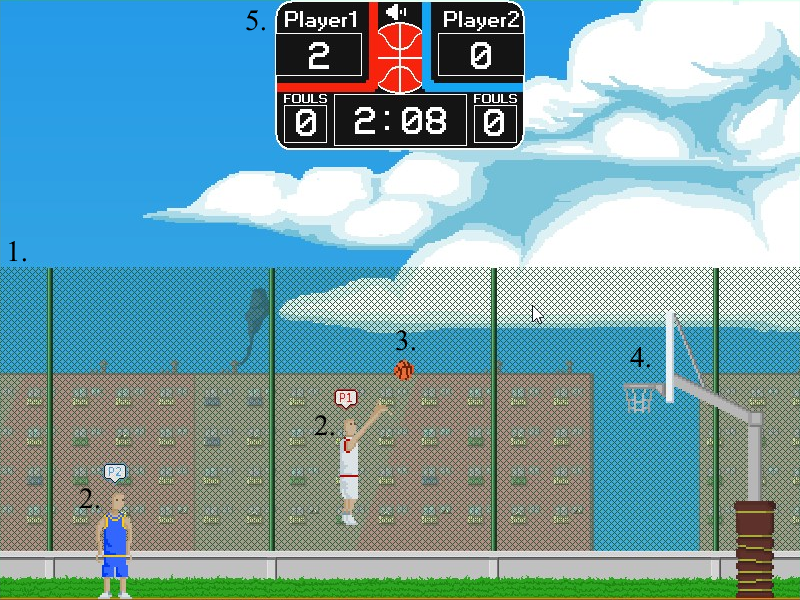
\includegraphics[scale=0.6]{\ImgPath/rys/game_elements.png}
\end{center}
	\caption{Elementy gry na zrzucie ekranu z aplikacji}
	\label{game_elements}
\end{figure}

\section{Inne funkcjonalności}
Wyżej wymienione elementy stanowią podstawę gry. Teoretycznie wystarczą one do przeprowadzenia pełnej rozgrywki jednak, nie wydaje się ona zbyt ciekawa. Gra posiada wiele funkcjonalności które ułatwiają rozgrywkę, zwiększają jej komfort, bądź też jej odczucie przez gracza:
\begin{itemize}
    \item Ekran ustawień - pozwala na ustawienie klawiszy które odpowiedzialne są za konkretne akcje w grze, oraz ustawienie poziomu głośności dźwięków. Ustawienia te są zapisywane w pliku .ini przez co po restarcie gry nie trzeba ich od nowa ustawiać. 
    \item Ekran ustawień meczu - pozwala na zmianę ustawień pojedynczego meczu. Zmienione może zostać:
    \begin{itemize}
        \item Czas meczu
        \item Wygląd postaci każdego z graczy
        \item Wygląd piłki
        \item Plansza
    \end{itemize}
    \item Dźwięki - zwiększają immersję i stanowią dodatkową informacje zwrotną z gry. W grze można usłyszeć dźwięki tła z plansz, uderzeń piłki o różne powierzchnie, gwizdka sygnalizujące faul, oraz dźwięki wyboru przycisku w menu.
    \item Efekty cząsteczkowe - Małe dodatki graficzne które sprawiają że gra wygląda ciekawiej. Można do nich zaliczyć efekt sypiącego się piasku gdy postać rusza. 
    \item Efekty specjalne - Głównie lekkie trzęsienie kamerą przy uderzeniach piłki o kosz. Stanowią dodatkową informacje zwrotną z gry.
    \item Dynamiczna kamera - Kamera która zawsze pokazuje w kadrze piłkę lub gracza z piłką. Gracz z piłką nie jest na środku, ponieważ kamera pokazuje zdecydowanie więcej strony w którą jest aktualnie zwrócony, tak żeby można było swobodnie rzucać.
    \item Obsługa padów - Gracze mogą nie chcieć używać klawiatury do gry z wielu powodów, dlatego też gra w pełni wspiera obsługiwanie jej tzw. padem czyli specjalnym kontrolerem stworzonym właśnie do grania w gry. Dzięki temu każdy gracz może wybrać swój preferowany sposób obsługi i nie musi dzielić klawiatury z przeciwnikiem.
    \item Osiągnięcia - Strona Gamejolt.com posiada system osiągnięć. Każdy użytkownik może je odblokować jeżeli zostały one zaimplementowane przez developera. W grze istnieją 3 osiągnięcia. Osiągnięcia są często ciekawym dodatkiem do gry i przedłużają czas jaki można spędzić                 nad grą.
    \item Znaczniki pozycji - Ponieważ postacie graczy nie zawsze są w kadrze, gracze nie posiadają informacji o swojej pozycji. Dzięki prostym strzałkom w kolorze gracza ta informacja jest zachowana. Ponadto, ponieważ możliwa jest zmiana wyglądu kontrolowanej postaci, a nawet możliwy jest wybór takiego samego wyglądu dla obu graczy, nad ich głowami widnieją znaczniki z numerem gracza.
\end{itemize}


\begin{figure}[!htbp]
	\begin{center}
\centering
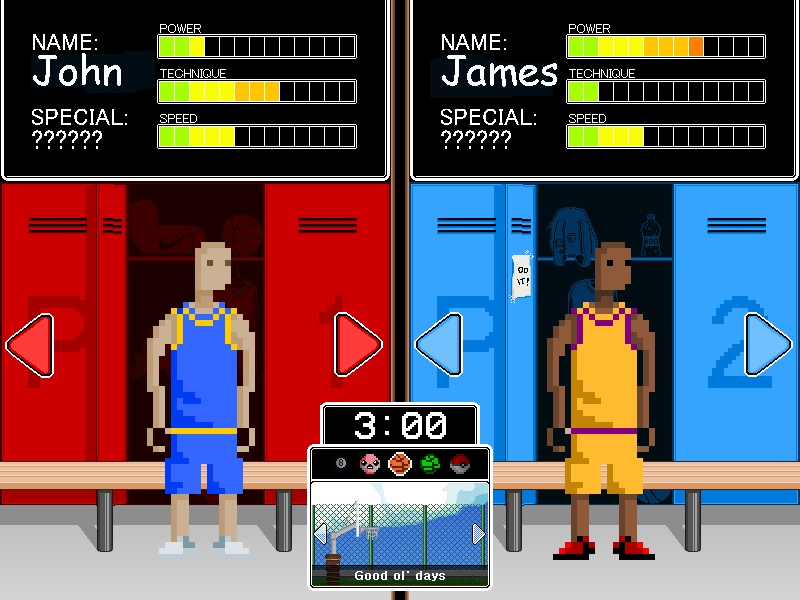
\includegraphics[scale=0.5]{\ImgPath/rys/match_setup_old.png}
\end{center}
	\caption{Ekran ustawień meczu}
	\label{match_setup_old}
\end{figure}


%-----------------
% Implementacja
%-----------------
\chapter{Implementacja nowej wersji gry}

\section{Zmiany w stosunku do oryginalnej wersji gry}

\section{Implementacja gry z wykorzystaniem środowiska Unity}

\section{Implementacja trybu online multiplayer}

\section{Przygotowanie gry pod nowe platformy}

%-----------------
% Testowanie
%-----------------
\chapter{Testowanie}


Ważne, pameitaj że w poprzednim roku na techniki multimedialne robiłeś samasymulacje piłki - były to ponieka testy.
\section{Przetestowanie opracowanej gry komputerowe}

\iffalse
%-----------------
% Steganografia
%-----------------
\chapter{Steganografia}
Wywodzące się z greki słowo ,,steganografia'' oznacza ,,ukryte pismo'' 
(\textit{steganos} - ukryty, tajny; \textit{graphein} - pisać, malować), co w 
odniesieniu do kanału informacyjnego oznacza przesyłanie danych w taki sposób, 
aby osoby postronne mające wgląd do danych nie mogły stwierdzić istnienia w nich 
ukrytej informacji. Cały mechanizm steganografii opiera się na zasadzie ukrycia 
informacji w tych częściach wiadomości, które nie służą do przekazywania 
informacji lub których modyfikacja nie wpływa na treść głównego przekazu.

W celu przesłania informacji za pomocą steganografii należy utworzyć kanał 
steganograficzny, zdefiniowany \cite{USDoD}  jako: ,,każdy kanał komunikacyjny, 
który może być wykorzystany przez stronę do przesłania informacji w sposób 
naruszający politykę bezpieczeństwa systemu''. Metoda ta wykorzystuje fakt 
przesłania danych w sposób i w miejscach, które zgodnie z protokołem do tego nie 
służą, narażając system na nieautoryzowany przesył informacji.

Steganografia w znaczącym stopniu różni się od kryptografii, która nie dba o 
zatajenie istnienia przekazu, a jedynie o jego integralność oraz uniemożliwienie 
stronom trzecim poznanie treści przekazu. Oczywiście najlepszą techniką jest 
połączenie steganografii z kryptografią. Takie podejście pozwala zabezpieczyć 
się przed sytuacją, w której strona nadzorująca transmisję, nawet w przypadku 
odkrycia przekazu steganograficznego nie może go odczytać ze względu na siłę 
zastosowanej kryptografii.
  %-----------------
  % Historia
  %-----------------
\section{Historia}
Pomimo, że pierwsze wzmianki o steganografii, a dokładnie o ukrytych kanałach w 
odniesieniu do systemów informatycznych notuje się na lata siedemdziesiąte XX 
wieku \cite{FirstCC}, to przykłady użycia steganografii sięgają starożytności. W 
literaturze powtarzają się opisy przekazywania tajnej informacji poprzez 
wytatuowanie jej na ogolonej głowie posłańca, który po odrośnięciu włosów był 
wysyłany z mało znaczącą wiadomością do armii swojego dowódcy. Każdy kto natknął 
się na posłańca miał wgląd do nieważnej wiadomości, niepodejrzewając nawet 
istnienia sekretnej informacji w postaci tatuażu.

Przykłady z historii odnoszą się także do bardziej współczesnych czasów. Wiele z 
metod steganografii było stosowanych podczas II Wojny Światowej (np. 
mikro-kropki) a także w latach Zimnej Wojny. Wiadomo także, że wielu agentów 
służb wywiadowczych, a szczególnie podwójnych agentów, przekazywało obcym 
państwom informację wykorzystując steganografię. Przykładem może tu być sprawa 
szpiega FBI Roberta Hanssena \cite{Hanssen}, który przy pomocy technik 
steganograficzny przez około dekadę przekazywał tajne informacje służbom KGB.

Rozdziały \ref{sectionSteganografiaWObiektachMultimedialnych} oraz 
\ref{chapterSteganografiaWRuchuTCPIP} opisują nowoczesne podejście do 
steganografii wykorzystujące współczesne kanały informacyjne. 
  %-----------------
  % Pojęcia
  %-----------------
\section{Pojęcia}
W celu zdefiniowania kanału steganograficznego oraz opisania transmisji z 
wykorzystaniem takiego kanału należy omówić jego części składowe:
\begin{itemize}
	\item dane do ukrycia, tajne dane - informacja jaką należy przesłać 
między uczestnikami komunikacji, tak aby strony trzecie nie miały do niej 
wglądu,
	\item dane nośne, wiadomość zakrywająca - wiadomość, w której ukryte 
zostaną tajne dane; przesyłanie wiadomości zakrywających musi być dozwolone w 
danym kanale informacyjnym i nie powinno wzbudzać podejrzeń,
	\item funkcja steganograficzna - funkcja przekształcająca dane do 
ukrycia oraz wiadomość zakrywającą w jedną połączoną wiadomość,
	\item dane z ukrytą wiadomością - dane zawierające ukrytą informację a 
jednocześnie wykazujące cechy danych nośnych,
	\item nadzorca komunikacji, wartownik - mechanizm mający pełen wgląd do 
wiadomości przekazywanej między stronami komunikacji, świadomy struktury 
komunikatów i potrafiący wykrywać występujące w nich anomalie,
	\item kanał komunikacyjny - kanał zestawiony pomiędzy nadawcą a 
odbiorcą, zapewniający przepływ informacji, do którego wgląd ma nadzorca 
komunikacji,
	\item odwrotna funkcja steganograficzna - funkcja przekształcająca dane 
z ukrytą wiadomością na tajne dane,
	\item klucz kryptograficzny - klucz znany tylko obu stronom komunikacji, 
służący do zabezpieczenia tajnej informacji metodami kryptografii symetrycznej 
przed ewentualnością złamania funkcji steganograficznej.
\end{itemize}
  %-----------------
  % Schemat komunikacji steganograficznej
  %-----------------
\section{Schemat komunikacji steganograficznej}
\label{sectionSchematKomunikacjiSteganograficznej}
Podstawowy scenariusz, powszechny w literaturze na temat steganografii, odnosi 
się do sytuacji opisanej w \cite{PrisonersProblem}. Dwóch więźniów (w naszym 
przypadku Alicja(\tech{A}) i Bob(\tech{B})) zamknięci są w dwóch odrębnych 
celach. Mogą się ze sobą kontaktować, jednak ich cała korespondencja przechodzi 
przez ręce Wartownika (\tech{W}). Ma on pełen wgląd do przekazywanych 
informacji, więc może przechwycić wszelkie przekazywane tajemnice, a dodatkowo w 
razie podejrzeń może nie dopuścić do komunikacji\footnote{podejrzana informacja 
jest tu analogią do stosowania kryptografii przez więźniów}. W takim przypadku w 
celu przekazania ważnych informacji \tech{A} i \tech{B} muszą posłużyć się 
pewnego rodzaju podstępem. Muszą tak sformułować treść przekazu, aby \tech{W} 
nie rozróżnił ,,niegroźnej'' wiadomości od wiadomości z ukrytym przekazem. 
Dlatego też przekazują wiadomość, w której prawdziwa treść możliwa jest do 
odczytania po złożeniu kolejno każdej np.  drugiej litery z każdego wyrazu.
\begin{figure}[!htbp]
	\begin{center}
\centering
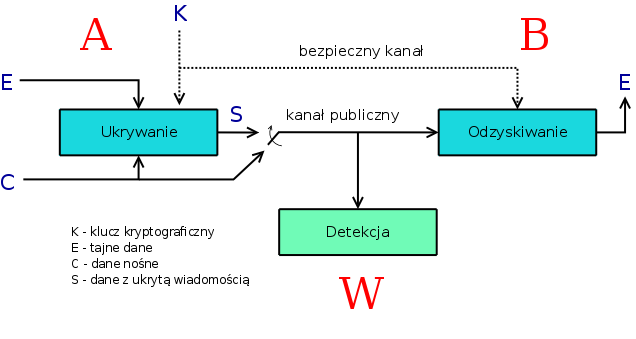
\includegraphics[scale=0.4]{\ImgPath/rys/schemat_komunikacji.png}
\end{center}
	\caption{Schemat komunikacji steganograficznej}
	\label{schematKomunikacji}
\end{figure}

Przedstawioną tak sytuację pokazuje rysunek 
\ref{schematKomunikacji}\footnote{sporządzony na podstawie 
\cite{schematKomunikacjiPrzypis}, rysunek 1, strona 3}. \tech{A} próbuje 
przesłać tajną informację \tech{E} do \tech{B}. Cała komunikacja odbywa się 
przez kanał publiczny, kontrolowany przez \tech{W}. W celu ukrycia faktu 
komunikacji \tech{A} stara się ukryć tajny przekaz w informacji \tech{C}. W celu 
uzyskania skutecznej steganografii \tech{W} nie może rozróżnić informacji 
poprawnej, nie zawierającej tajnych danych, od informacji \tech{S}, która 
zawiera tajną informację. W celu dodatkowego zabezpieczenia przekazu, \tech{A} i 
\tech{B} mogą korzystać z funkcji kryptograficznej zabezpieczającej przekazywane 
informacje. Można tu wykorzystać metody kryptografii symetrycznej (ustalony 
klucz kryptograficzny \tech{K}) lub niesymetrycznej (klucz publiczny 
\tech{K}$_{pub}$ i klucz prywatny \tech{K}$_{pryw}$).

Stosowanie technik kryptograficznych wpływa na poprawę bezpieczeństwa 
przesyłanej informacji, jednak należy pamiętać o nieporządnych cechach jakie 
mogą one wywołać. W większości przypadków umieszczenie tajnej informacji 
steganograficznej w przekazie wiąże się z zamianą istniejącej już nieważnej 
części informacji. Jednak każda porcja usuniętej informacji może mieć pewną 
charakterystyczną postać lub specyficzny histogram. Zastosowanie funkcji 
kryptograficznej w stosunku do tajnej informacji zmienia ją, a wynikowy rozkład 
bitów jest nieprzewidywalny i w większości przypadków różny od standardowych 
histogramów określonych dla podmienianych części wiadomości.
  %-----------------
  % Stegoanaliza
  %-----------------
\section{Stegoanaliza}
Stegoanaliza to nauka zajmująca się wykrywaniem istnienia ukrytych informacji w 
kanałach komunikacyjnych. Nie zawsze prowadzi to do odkrycia dokładnej treści 
ukrytego przekazu, a w większości przypadków polega jedynie na wskazaniu 
istnienia ukrytego kanału steganograficznego.

Możliwość wykrycia kanału steganograficznego sprowadza się do analizy różnych 
części wiadomości lub strumienia danych w celu wykrycia anomalii. Takie 
podejście wynika z faktu, że tajna informacja ukryta jest w miejscach nie 
przeznaczonych do przesyłania informacji lub na miejscu danych, które są w 
pewien sposób nadmiarowe (np. dla zmysłów człowieka). Można wskazać dwa 
podstawowe sposoby wykrywania anomalii:
\begin{itemize}
	\item pierwsze podejście opiera się na przebadaniu wszystkich części 
informacji (np. pól nagłówka TCP/IP), których struktura jest w pełni 
przewidywalna lub których wartości są zdefiniowane przez standardy lub 
powszechne praktyki; ważne jest także sprawdzenie czy występują wartości 
nadmiarowe oraz czy elementy sygnalizujące wystąpienie dodatkowych danych mają 
faktyczne pokrycie w danych,
	\item drugą metodą jest porównanie wartości części wiadomości (np. pól 
nagłówka TCP/IP) i zaklasyfikowanie ich jako prawdopodobnych lub nie dla danego 
systemu bądź protokołu; takie podejście może być stosowane do wartości ściśle 
określonych, takich jak wymienione w pierwszym punkcie, jednak można je także 
stosować do wartości które są pseudolosowe lub których histogram jest 
charakterystyczny; w celu realizacji tej metody warto posłużyć się sieciami 
neuronowymi takimi jak SVM i RSVM, zdolnymi rozpoznawać wzorce i separować dane.
\end{itemize}
  %-----------------
  % Metody tworzenia steganografii
  %-----------------
\section{Metody tworzenia steganografii oraz rodzaje ukrytych kanałów}
Przesłanie danych za pomocą przekazu steganograficznego wiąże się w większości 
przypadków z umieszczeniem dodatkowej informacji w wiadomości. Odbywa się to za 
pomocą podmiany tej części wiadomości (nagłówka TCP/IP), która wykazuje cechy 
nadmiarowości lub której (kontrolowana) zmiana nie prowadzi do przerwania 
transmisji. Pewną podgrupą może być w tym przypadku wykorzystanie pól 
oryginalnie pustych (zerowych) lub niewykorzystywanych w istniejących 
implementacjach.

Kanały steganograficzne można podzielić na dwa zasadniczne 
typy\cite{SweetyPresentation}:
\begin{itemize}
	\item kanał pojemnościowy (ang. storage channel) - informacja zawarta w 
częściach wiadomości, polach nagłówka,
	\item kanał czasowy (ang. timing channel) - informacja zawarta w czasach 
wystąpienia danych zdarzeń, np. przesłania pakietu TCP/IP.
\end{itemize}
W przypadku sieci pakietowych można także połączyć dwa typu kanałów 
steganograficznych, tworząc kanał mieszany, w którym jeden z typów (np. 
pojemnościowy) będzie wykorzystywany do przekazywania informacji, a drugi (np. 
czasowy) do sygnalizacji tego zdarzenia.

Większość opracowanych programów służących do przesyłania danych z 
wykorzystaniem steganografii opiera się na kanałach pojemnościowych. Wynika to z 
faktu, że kanały czasowe narzucają pewne ograniczenia na generację pakietów 
TCP/IP przez co ich wykrycie staje się prostsze.

Dodatkowo należy zauważyć, że w sieciach pakietowych można skonstruować 
abstrakcyjny kanał steganograficzny, w którym do przesyłania tajnych danych 
lub/i obsługi protokołu steganograficznego wykorzystywane są różne pola 
nagłówka. Zmiana wykorzystania danego pola może być dynamiczna, zależna od 
wymaganej przepustowości lub w celu zminimalizowania wykrycia kanału 
steganograficznego. 
  %-----------------
  % Cechy kanału steganograficznego
  %-----------------
\section{Cechy kanału steganograficznego}
Każdy kanał steganograficzny posiada trzy cechy, które decydują o jego 
przydatności w danej sytuacji:
\begin{enumerate}
	\item pojemność (przepustowość) - określa jaką porcję informacji możemy 
przesłać w danej wiadomości nośnej; w przypadku steganografii w TCP/IP, wyrażana 
jest w bitach na sekundę, bitach na pakiet lub bitach na sesję TCP; 
przepustowość odgrywa ważną rolę w przypadku konieczności przekazania dużej 
ilości informacji, jednak należy pamiętać, że to przeważnie prowadzi do 
ułatwionej detekcji steganografii,
	\item bezpieczeństwo - określa jak łatwo jest uzyskać dostęp do 
przekazywanej tajnej informacji w przypadku poznania mechanizmu tworzenia 
przekazu steganograficznego; dodatkowym mechanizmem zwiększającym bezpieczeństwo 
może być używanie znanych tylko sobie zmiennych pseudolosowych lub modyfikacji 
algorytmu\footnote{jest to znane jako ,,bezpieczeństwo przez zatajenie'' (ang. 
security through obscurity) i powinno być używane tylko jako dodatkowy element 
systemu zabezpieczeń},
	\item krzepkość (ang. robustness) - określa stopień w jakim możemy 
zmodyfikować przekaz nie uszkadzając zawartej w nim informacji 
steganograficznej; niestety w przypadku steganografii naruszenie kanału (pola) 
zawierającego przekaz steganograficzny przeważnie wiąże się z utratą tajnego 
przekazu.
\end{enumerate}

  %-----------------
  % Steganografia w obiektach multimedialnych
  %-----------------
\section{Steganografia w obiektach multimedialnych}
\label{sectionSteganografiaWObiektachMultimedialnych}
Pomimo, że steganografia ma zastosowanie prawie w każdej formie komunikacji, w 
latach 90-tych zyskała ona powodzenie jako technika ukrywania informacji w 
obiektach multimedialnych. Wynika to przede wszystkim z powszechności tego 
rodzaju przekazu, jego rozmiarów oraz prostoty obsługi programów do ukrywania 
informacji w obiektach multimedialnych, takich jak obraz, dźwięk i wideo. 
Dodatkowym atutem przy zastosowaniu tych metod jest stosunek ukrytej informacji 
do oryginalnego przekazu, sięgający w ekstremalnych sytuacjach 50\%, bez 
zauważalnego pogorszenia się jakości przekazywanych danych.

Użycie steganografii w treściach multimedialnych sprowadza się do takiego 
manipulowania danymi, aby plik wynikowy zawierał dodatkowe informacje, a 
jednocześnie nie był rozróżniany przez zmysły człowieka w porównaniu z 
oryginałem.

Jedną z najszerzej omawianych form steganografii w obiektach multimedialnych 
jest ukrywanie informacji w plikach graficznych. Istnieje wiele rozwiązań, 
zarówno bezpłatnych, o otwartym kodzie jak i komercyjnych. Przykładami mogą tu 
być takie programy jak Outguess, JPHide, StegHide. Istnieją różne techniki 
ukrywania informacji w plikach graficznych. Najprostszym rozwiązaniem jest 
podmiana najmniej znaczących bitów opisujących kolor danego piksela. Możliwe 
jest też zastosowanie dyskretnej transformaty kosinusowej.

W przypadku wybrania jako wiadomości nośnej pliku audio, możemy także zastosować 
metodę podmiany najmniej znaczących bitów. Dodatkowo stosowane są metody 
ukrywania tajnych wiadomości poprzez rozszerzanie spektrum danego nagrania, czy 
też dodawanie echa. Przykładem narzędzia do tworzenia wiadomości 
steganograficznych może być UnderMP3Cover, MP3Stego czy 
S-Tools\footnote{\url{http://www.stegoarchive.com}}.

Kolejnym przykładem wykorzystania jako pliku nośnego obiektu multimedialnego 
jest plik wideo. Dodatkowa informacja może być przekazana przy użyciu dyskretnej 
transformaty kosinusowej. Jako przykładowe implementacje można podać StegoVideo.

Istnieje kilka technik umożliwiających wykrycie lub usunięcie steganografii 
zastosowanej w obiektach multimedialnych. Pierwszym podejściem, choć przeważnie 
trudnym do zastosowania, jest użycie oryginalnego pliku jako wzorca do 
porównania z przechwyconą wersją. W przypadku plików graficznych lub wideo 
możliwe jest użycie analizatorów statystycznych, które mogą wykryć anomalie 
występujące w histogramach tych wiadomości.

Zamiast wykrywać istnienie steganografii, częstym podejściem jest jej 
ograniczanie lub ,,ślepe'' usuwanie z wiadomości tych danych, które mogą być 
nośnikiem kanału steganograficznego. W przypadku plików multimedialnych 
najlepszym sposobem uzyskania takiego efektu jest przekodowanie pliku na inny 
standard i powrót do standardu wejściowego. Przeważnie zmiany w jakości plików 
są niezauważalne, a użycie konwersji sprowadza się do takiej zmiany bitów, która 
niszczy zawartą w nich steganografię.

W przypadku plików multimedialnych użycie steganografii jest pomocne w ochronie 
praw autorskich, przez stosowanie jej jako cyfrowych znaków wodnych. Niestety, 
tak jak zostało to wcześniej przedstawione w trakcie konwersji wiele z 
zakodowanej informacji ginie bezpowrotnie. Skutkiem tego może być pogorszenie 
jakości pliku multimedialnego, ale także usunięcie z niego cyfrowego znaku 
wodnego.

Itd., itd., itd. ...

\chapter{Steganografia w ruchu TCPIP}
\label{chapterSteganografiaWRuchuTCPIP}

Itd., itd., itd ...
\fi
%-----------------
% Podsumowanie i wnioski 
%-----------------
\chapter{Podsumowanie i wnioski }

\iffalse
Protokół TCP/IP jest najbardziej rozpowszechnionym i używanym protokołem 
komunikacji między systemami w sieci Internet oraz w sieciach intranet. Niestety 
został on opracowany na początku lat siedemdziesiątych, gdy problemy 
bezpieczeństwa informacji nie stały na pierwszym miejscu. Ciągły wzrost działań 
przestępczych w sieci Internet, w tym wymiana nielegalnych treści, prowadzi do 
stosowania coraz to nowszych technik zabezpieczających. Z tego względu obserwuje 
się działania mające na celu wprowadzenie tajnej komunikacji między przejętymi 
systemami, tak aby nie wzbudzić ostrzeżeń w analizatorach sieciowych. Taka 
ukryta komunikacja odbywa się z wykorzystaniem steganografii.

Wprowadzenie steganografii do niskich warstwach stosu TCP/IP umożliwia obejście 
wielu filtrów nałożonych na warstwy wyższe. Większość sieci oparta jest na 
protokołach rodziny TCP/IP, przez co nie można zabronić ich używania. Możliwa 
jest jedynie kontrola poprawności semantyki protokołów TCP/IP, a także 
ewentualna ingerencja w przekazywane wartości, z uwzględnieniem stanowości 
niektórych pól.

Opracowany schemat generacji początkowych numerów sekwencyjnych w jak najlepszy 
sposób odzwierciedla oryginalny proces zachodzący w stosie sieciowym systemu 
Linux. W większości przypadków występujących w rzeczywistych sieciach i 
systemach, numery wygenerowane przy pomocy \tech{Shushi} nie byłyby rozróżnialne 
od numerów wygenerowanych przez stos sieciowy systemu.

Jeżeli proces generacji wartości użytych do przekazania danych 
steganograficznych zostanie oparty o oryginalne mechanizmy używane do ich 
generacji, to pasywny analizator sieciowy nie będzie w stanie wykryć istnienia 
anomalii. Różnice możliwe są do zaobserwowania w przypadku zaistnienia 
specyficznych sytuacji występujących dla danej implementacji protokołu. W 
przypadku zastosowania pasywnego analizatora wymaga to jednak oczekiwania na 
taką sytuację. Z przeprowadzonych testów wynika, że lepszym podejściem jest 
zastosowanie analizatorów aktywnych, które posiadają wiedzę na temat testowanych 
systemów oraz ich chrakterystycznych cech implementacji. Skonstruowanie takiego 
analizatora jest zadaniem stosunkowo prostym a daje bardzo wysoką skuteczność.

Z przeprowadzonych testów wynika, że celowe jest prowadzenie dalszych prac w 
następujących obszarach:
\begin{itemize}
 \item dokładniejszy mechanizm generacji wartości mikrosekund
 \item wprowadzenie algorytmów zdolnych wykryć i uniemożliwić działanie 
analizatora aktywnego
\end {itemize}

Jeżeli powyższe punkty nie zostaną spełnione, analizatory aktywne będą w stanie 
wykryć istnienie modułu steganograficznego opartego na początkowych numerach 
sekwencyjnych.

\begin{tabular}{c|cc}
pierwsza kolumna & druga & trzecia \\ \hline
1 & 2 & 3 \\
a & b & c \\
\end{tabular} 

\begin{equation}
 E = m c^2 \label{einstein}
\end{equation}

Rozwój opracowanego rozwiązania steganograficznego jest możliwy poprzez 
wprowadzenie elementów  -- patrz wzór (\ref{einstein}) -- jak:
\begin{itemize}
 \item obsługa innych, przyszłościowych protokołów sieciowych, takich jak SCTP 
(ang. Stream Control Transmission Protocol)\cite{RFC2960}
 \item zapewnienie dwustronnej komunikacji z wykorzystaniem numerów 
potwierdzenia \tech{ACK}
 \item przeniesienie implementacji do innych systemów operacyjnych
\end{itemize}

Wraz ze wzrostem przepustowości urządzeń sieciowych (obecnie 10Gb/s i więcej) 
wzrasta problem analizy przepływających danych w czasie rzeczywistym. 
Analizatory sieciowe muszą w coraz krótszym czasie zbadać coraz większy strumień 
danych (miliony pakietów na sekundę). Jednak problem wzrostu prędkości sieci 
utrudnia zadanie także osobom implementującym kanały steganograficzne w 
protokole TCP/IP. Coraz więcej operacji wyższych warstw stosu sieciowego 
przenoszonych jest do układów scalonych interfejsów sieciowych. Taka technologia 
znana jest pod skrótem TOE (ang. TCP Offload Engine) i odnosi się przede 
wszystkim do sprzętowej generacji sum kontrolnych oraz mechanizmu TSO (ang. TCP 
segmentation offload). W następnych latach spodziewane jest przenoszenie 
kolejnych elementów stosu sieciowego TCP/IP do implementacji sprzętowych.

Ze względu na rozwój systemów zabezpieczających ruch sieciowy oraz wzrost 
bezpieczeństwa systemów operacyjnych, w kolejnych latach wzrośnie także 
wykorzystanie technik steganograficznych przez grupy przestępcze działające w 
ramach Internetu. Z tego powodu poznanie technik steganograficznych oraz 
wypracowanie metod obrony i wykrywania takiej komunikacji jest bardzo ważne.
\fi
%-----------------
% Dodatki 
%-----------------
\appendix
\iffalse
\chapter{Porównanie numerów ISN jądra Linux i modułu Shushi}
\begin{figure}[!htbp]
	\begin{center}
\centering
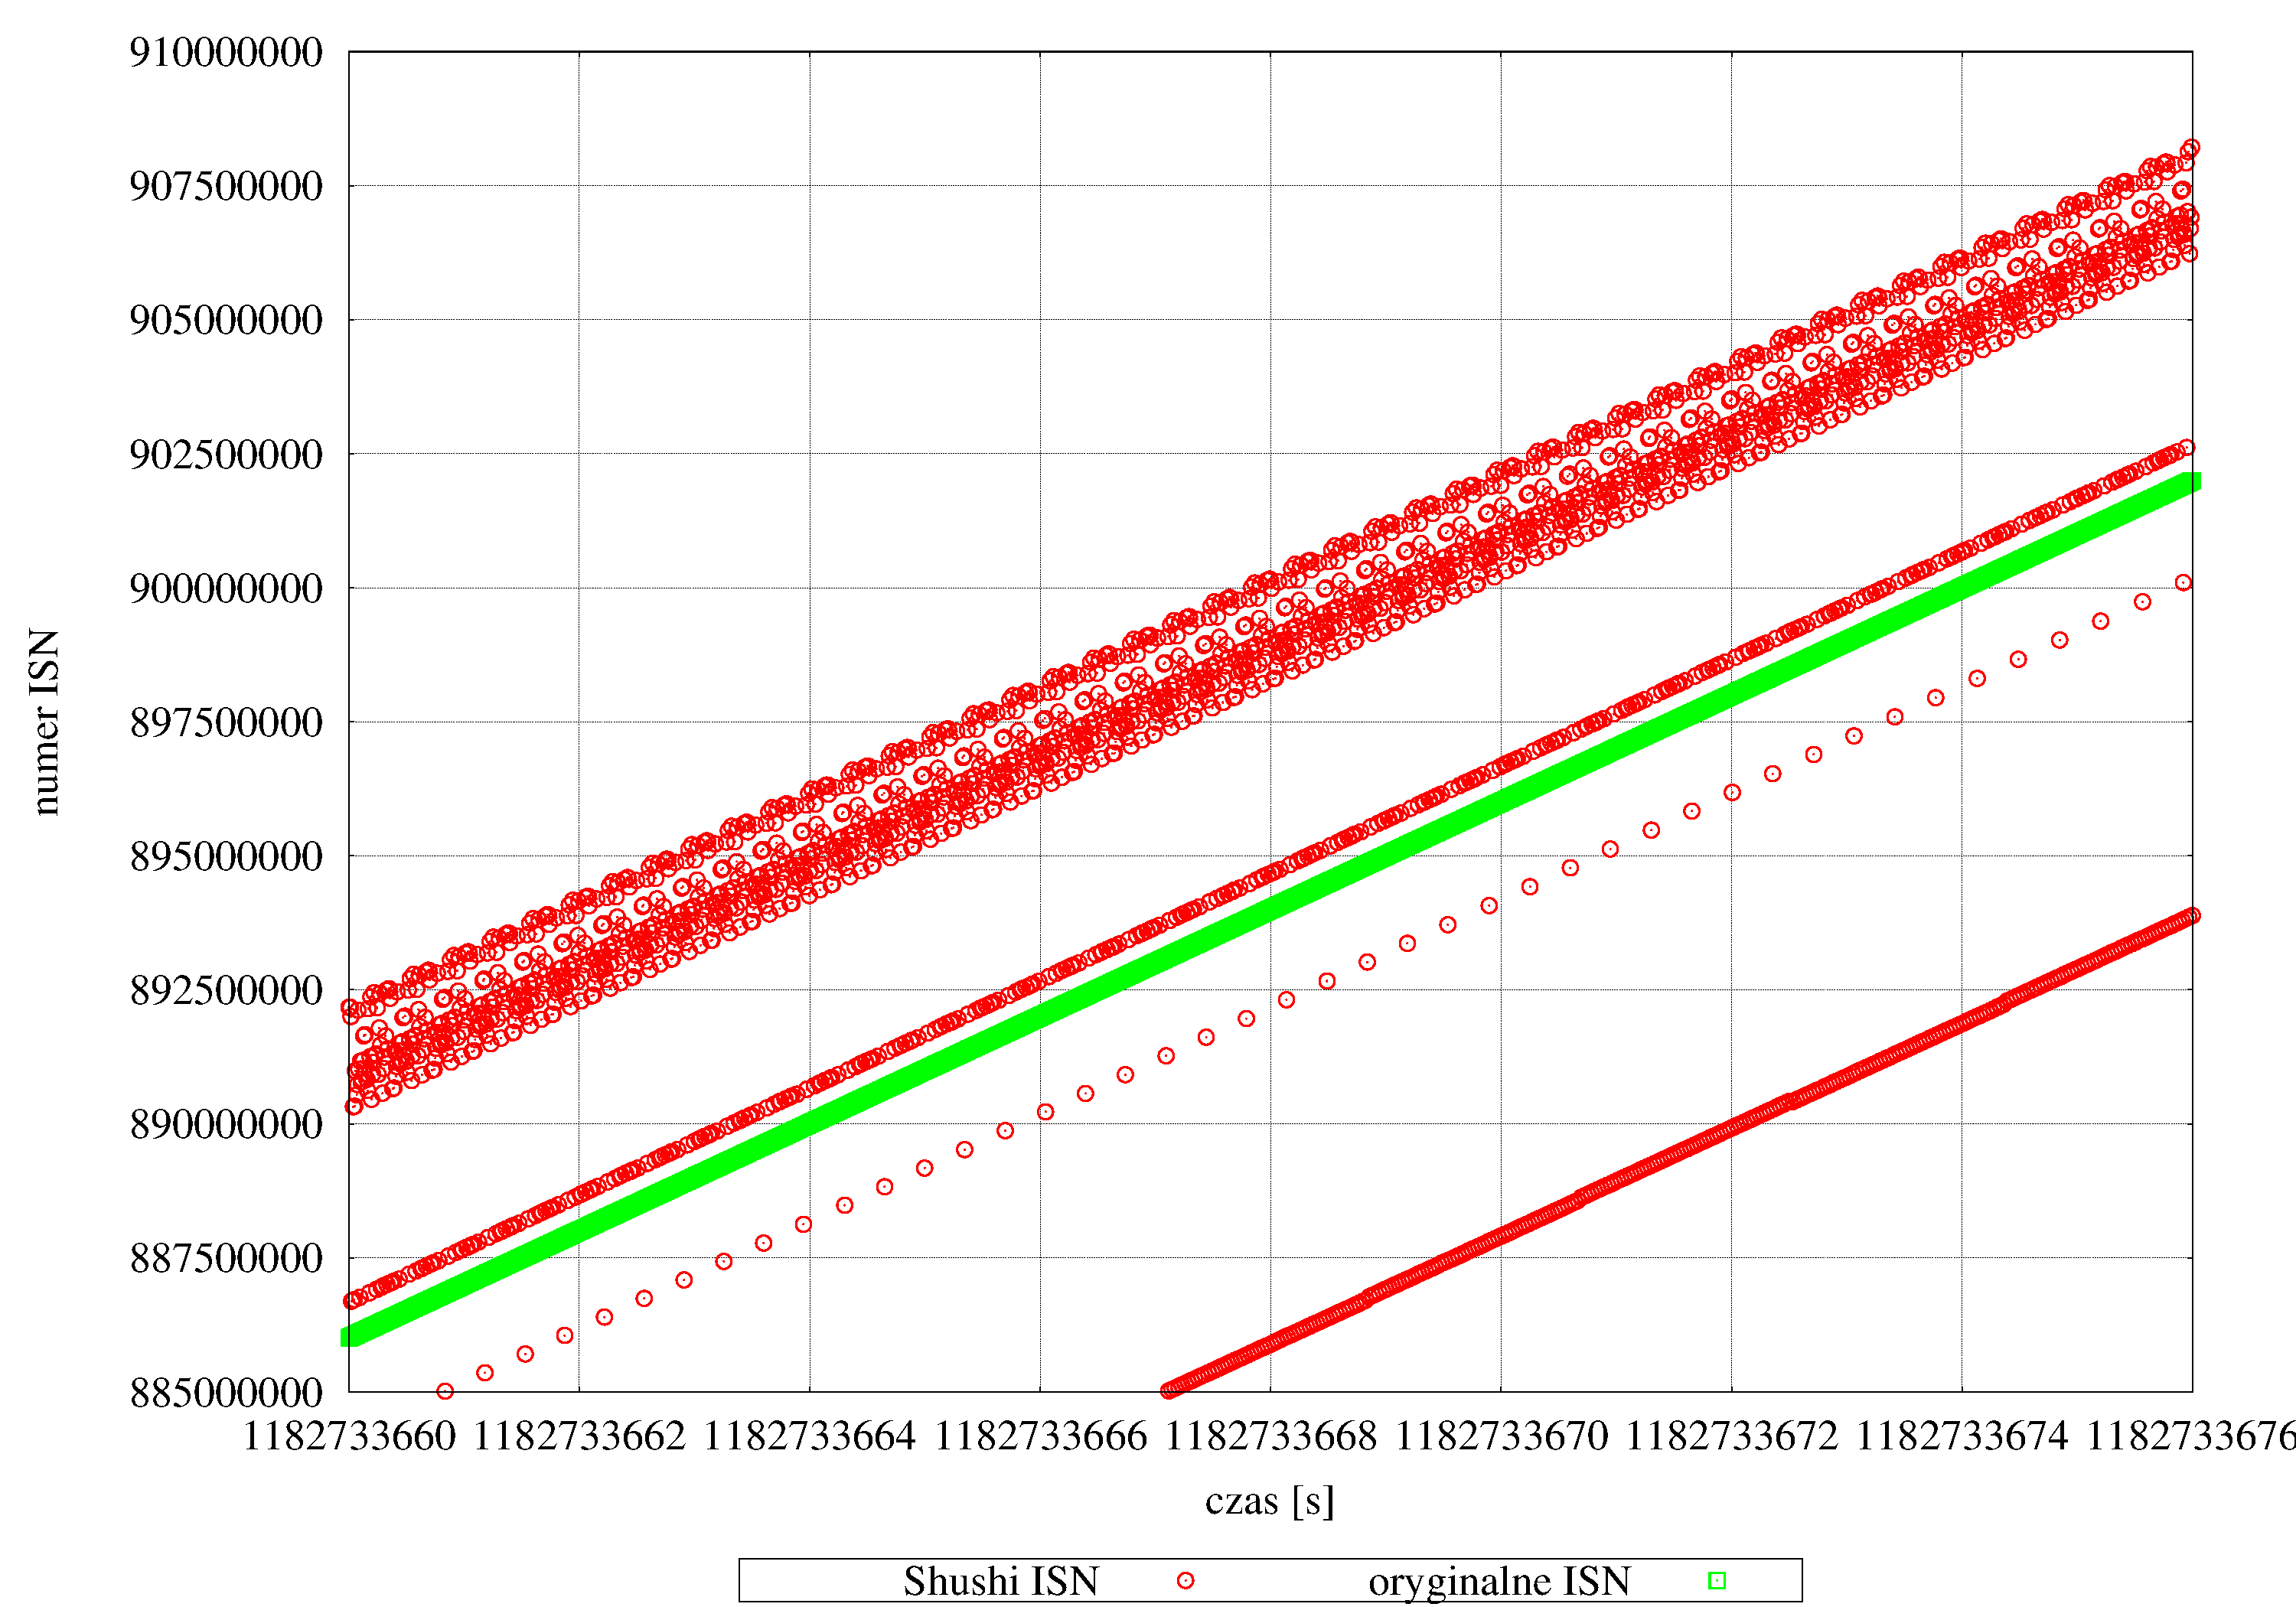
\includegraphics[scale=0.21]{\ImgPath/rys/IPPortConstData.pdf}
\end{center}
	\caption{Numery ISN wygenerowane przez jądro oraz \tech{Shushi}, stałe 
numery IP oraz porty TCP, stałe dane dla \tech{Shushi}, serie po około 2800 
próbek.}
	\label{IPPortConstData}
\end{figure}

\begin{figure}[!htbp]
	\begin{center}
\centering
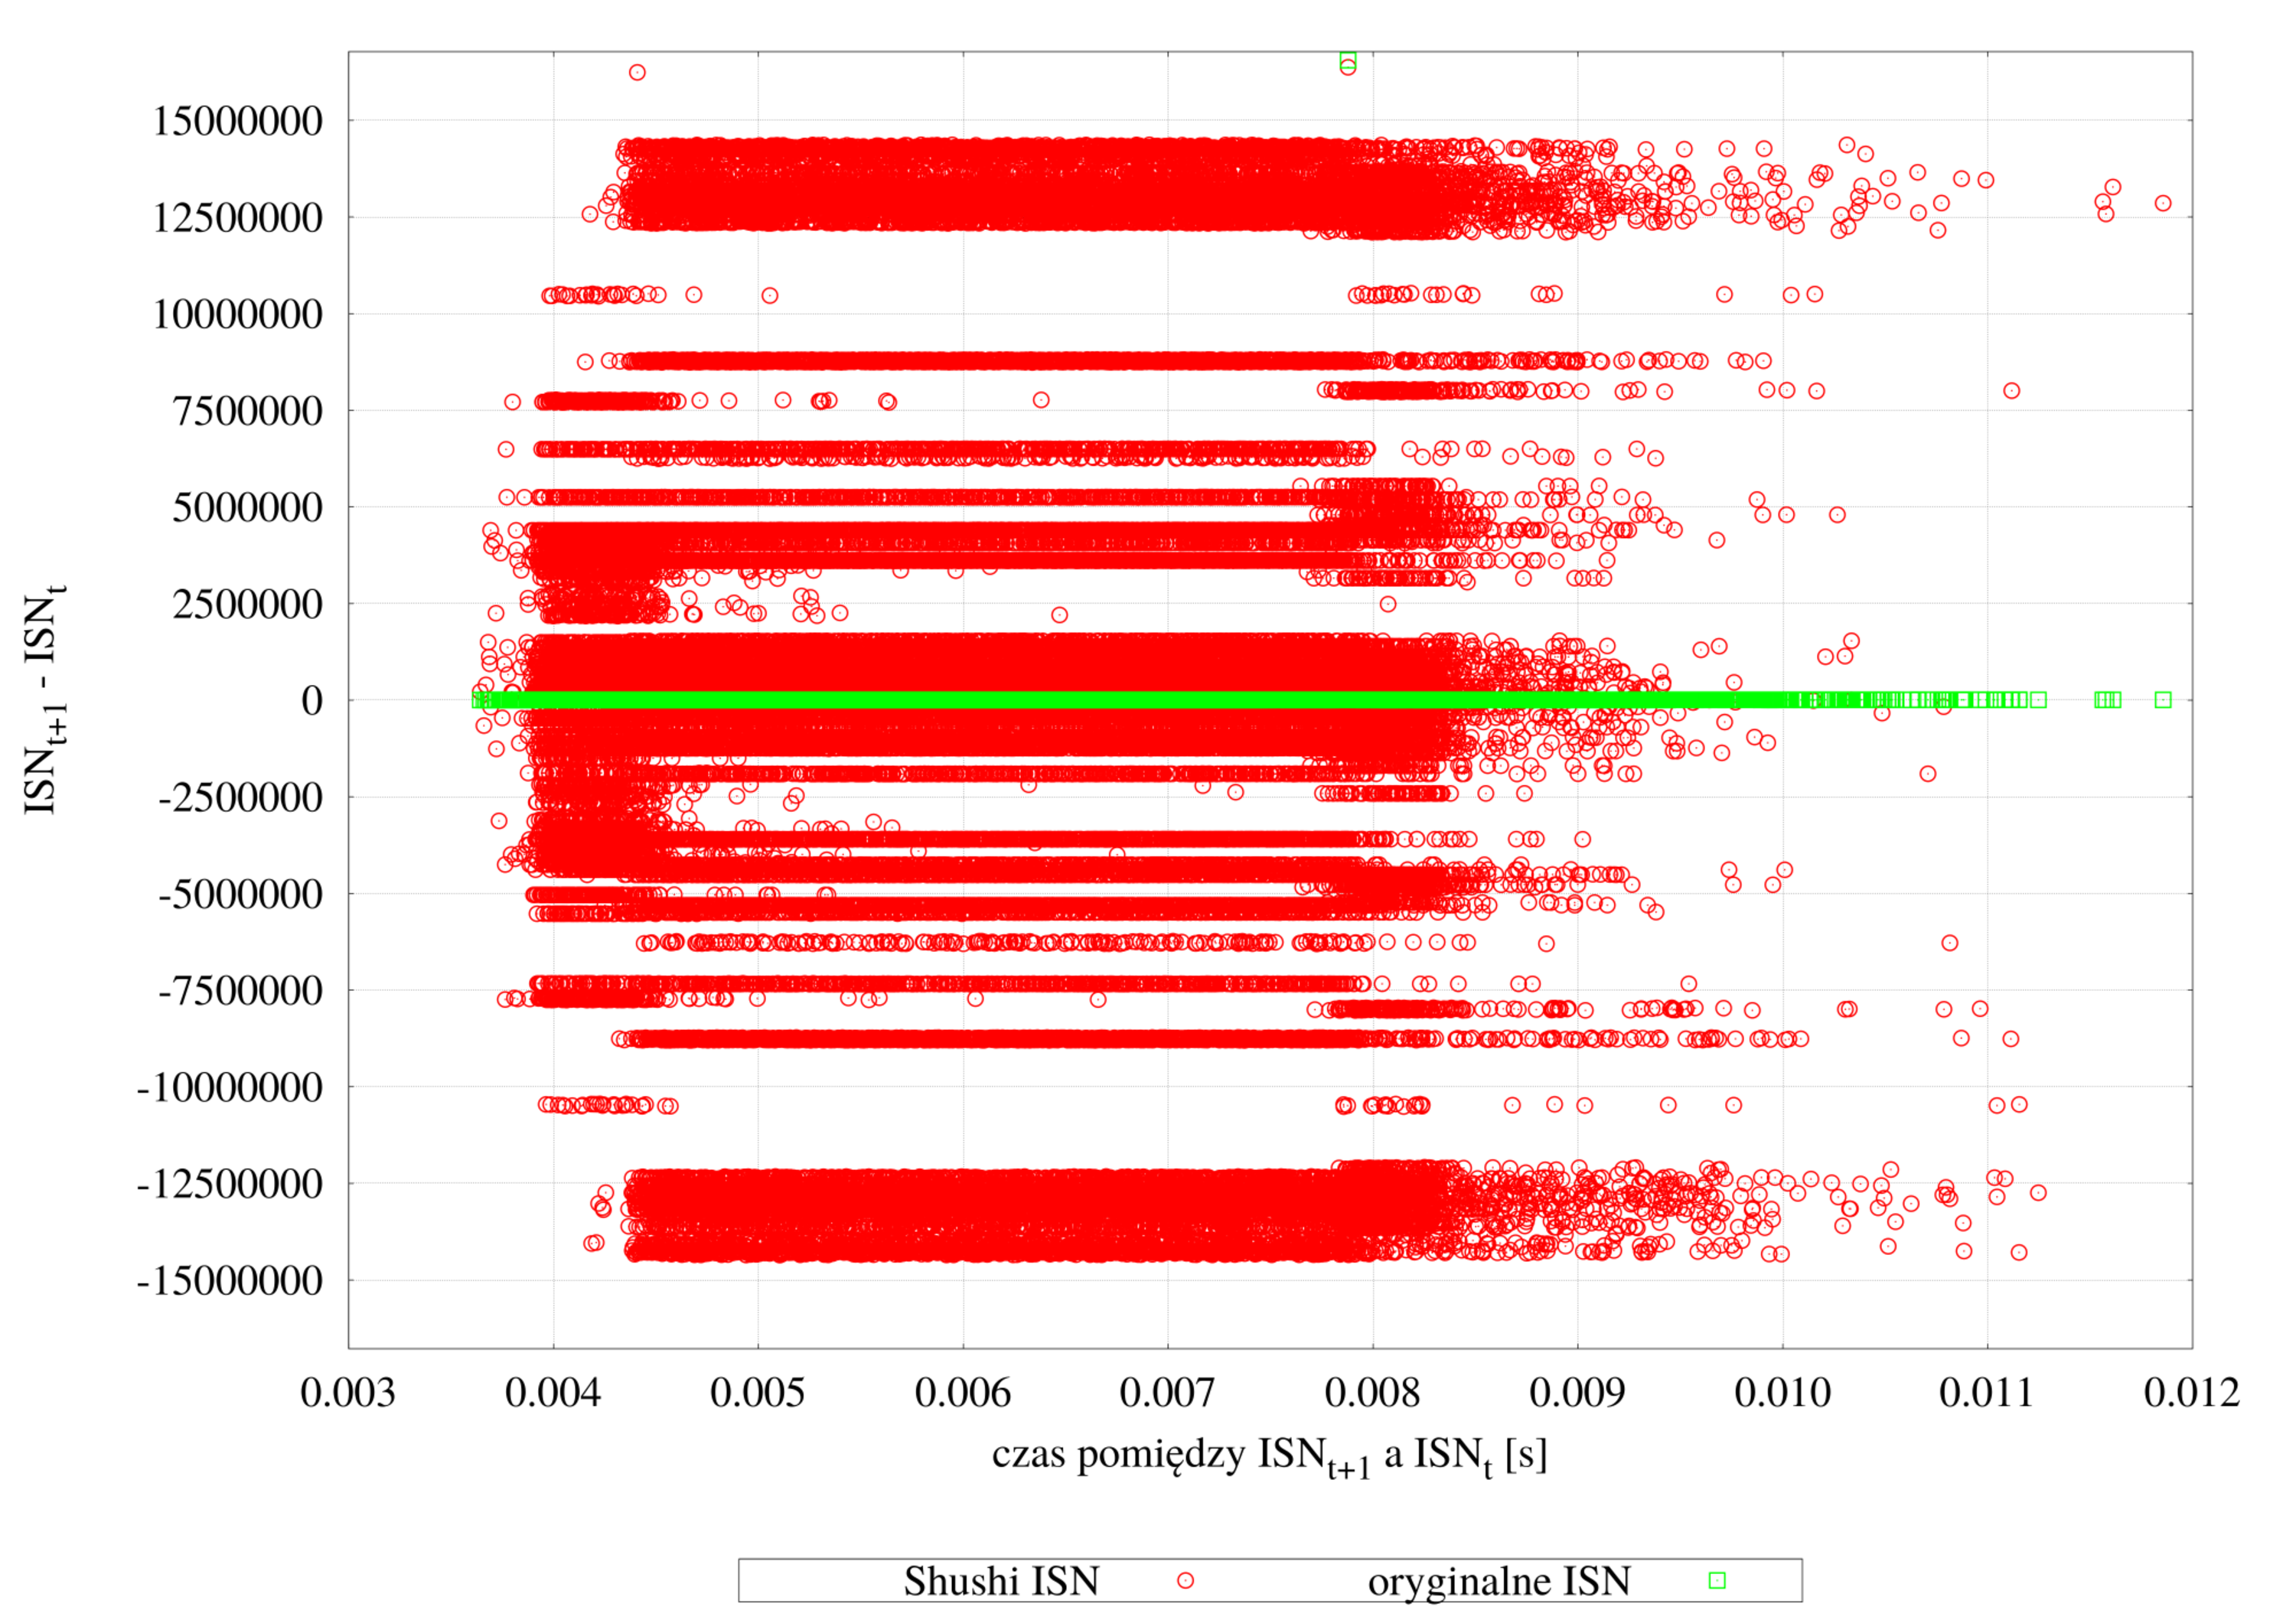
\includegraphics[scale=0.21]{\ImgPath/rys/IPPortConstDataDiff.pdf}
\end{center}
	\caption{Różnice pomiędzy kolejnymi numerami ISN wygenerowanymi przez 
jądro oraz \tech{Shushi}, stałe numery IP oraz porty TCP, stałe dane dla 
\tech{Shushi}, serie po około 60000 próbek.}
	\label{IPPortConstDataDiff}
\end{figure}

\begin{figure}[!htbp]
	\begin{center}
\centering
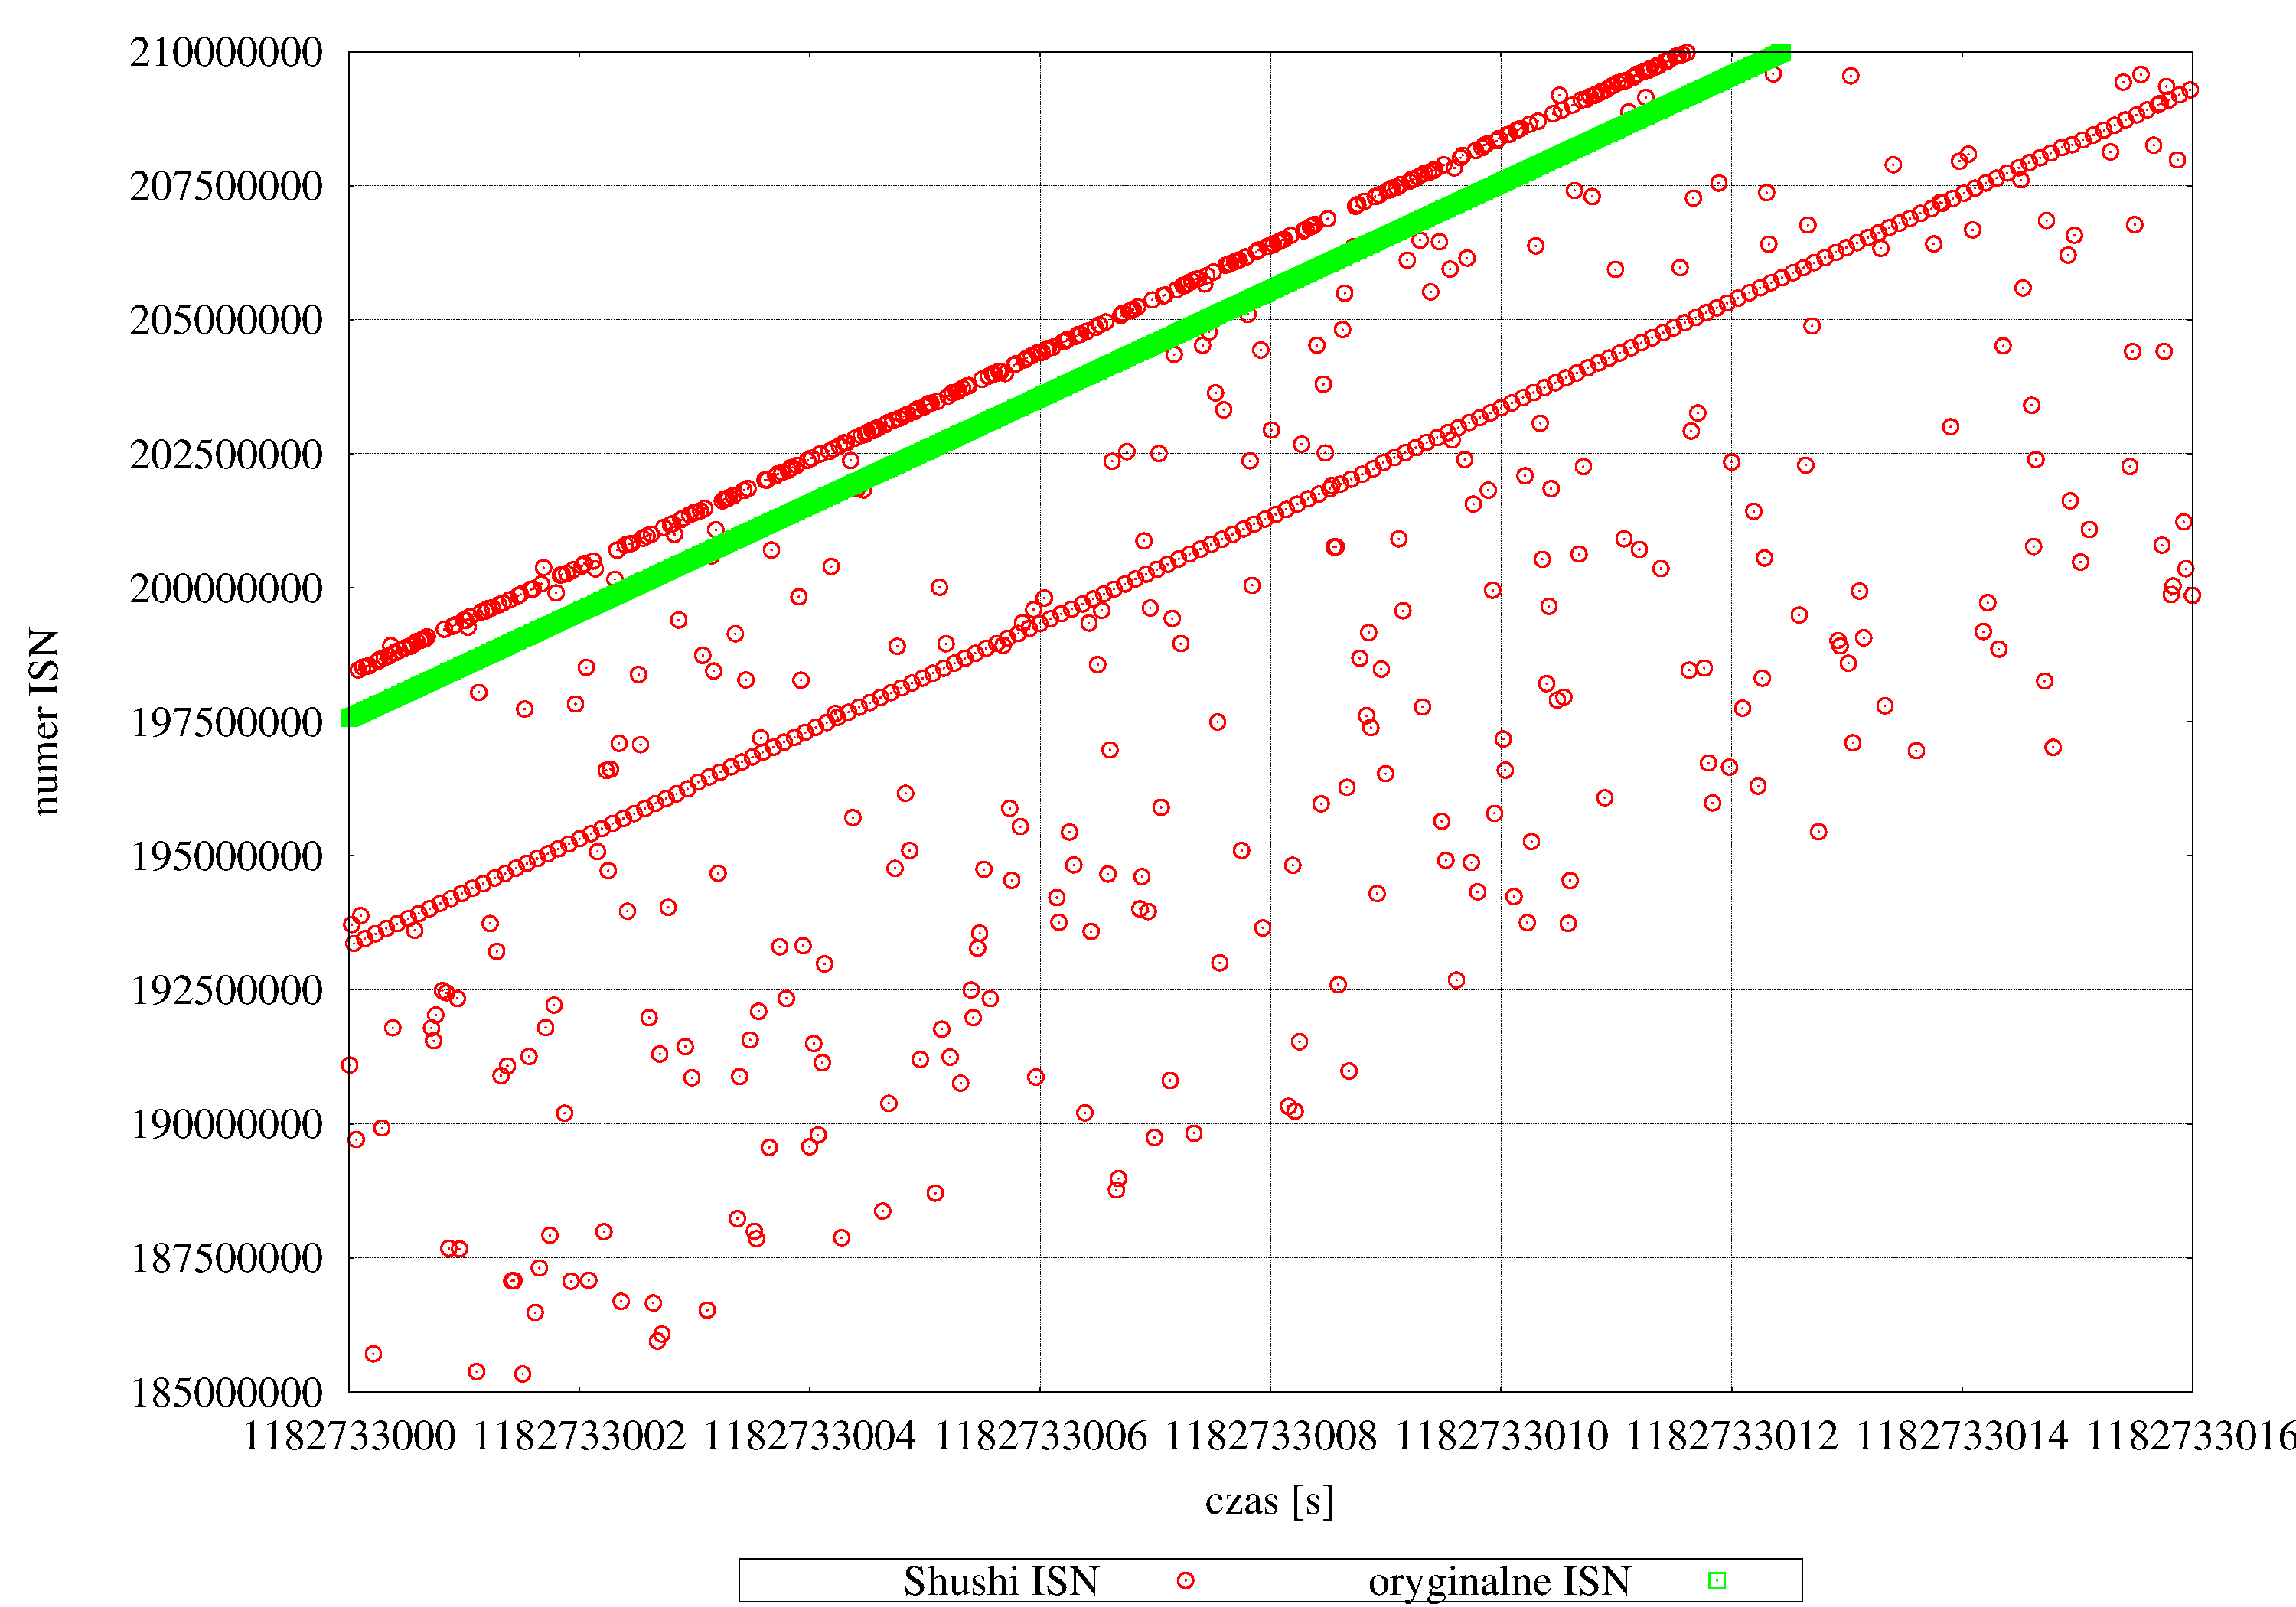
\includegraphics[scale=0.21]{\ImgPath/rys/IPPortRandData.pdf}
\end{center}
	\caption{Numery ISN wygenerowane przez jądro oraz \tech{Shushi}, stałe 
numery IP oraz porty TCP, losowe dane dla \tech{Shushi}, serie po około 860 
próbek.}
	\label{IPPortRandData}
\end{figure}

\begin{figure}[!htbp]
	\begin{center}
\centering
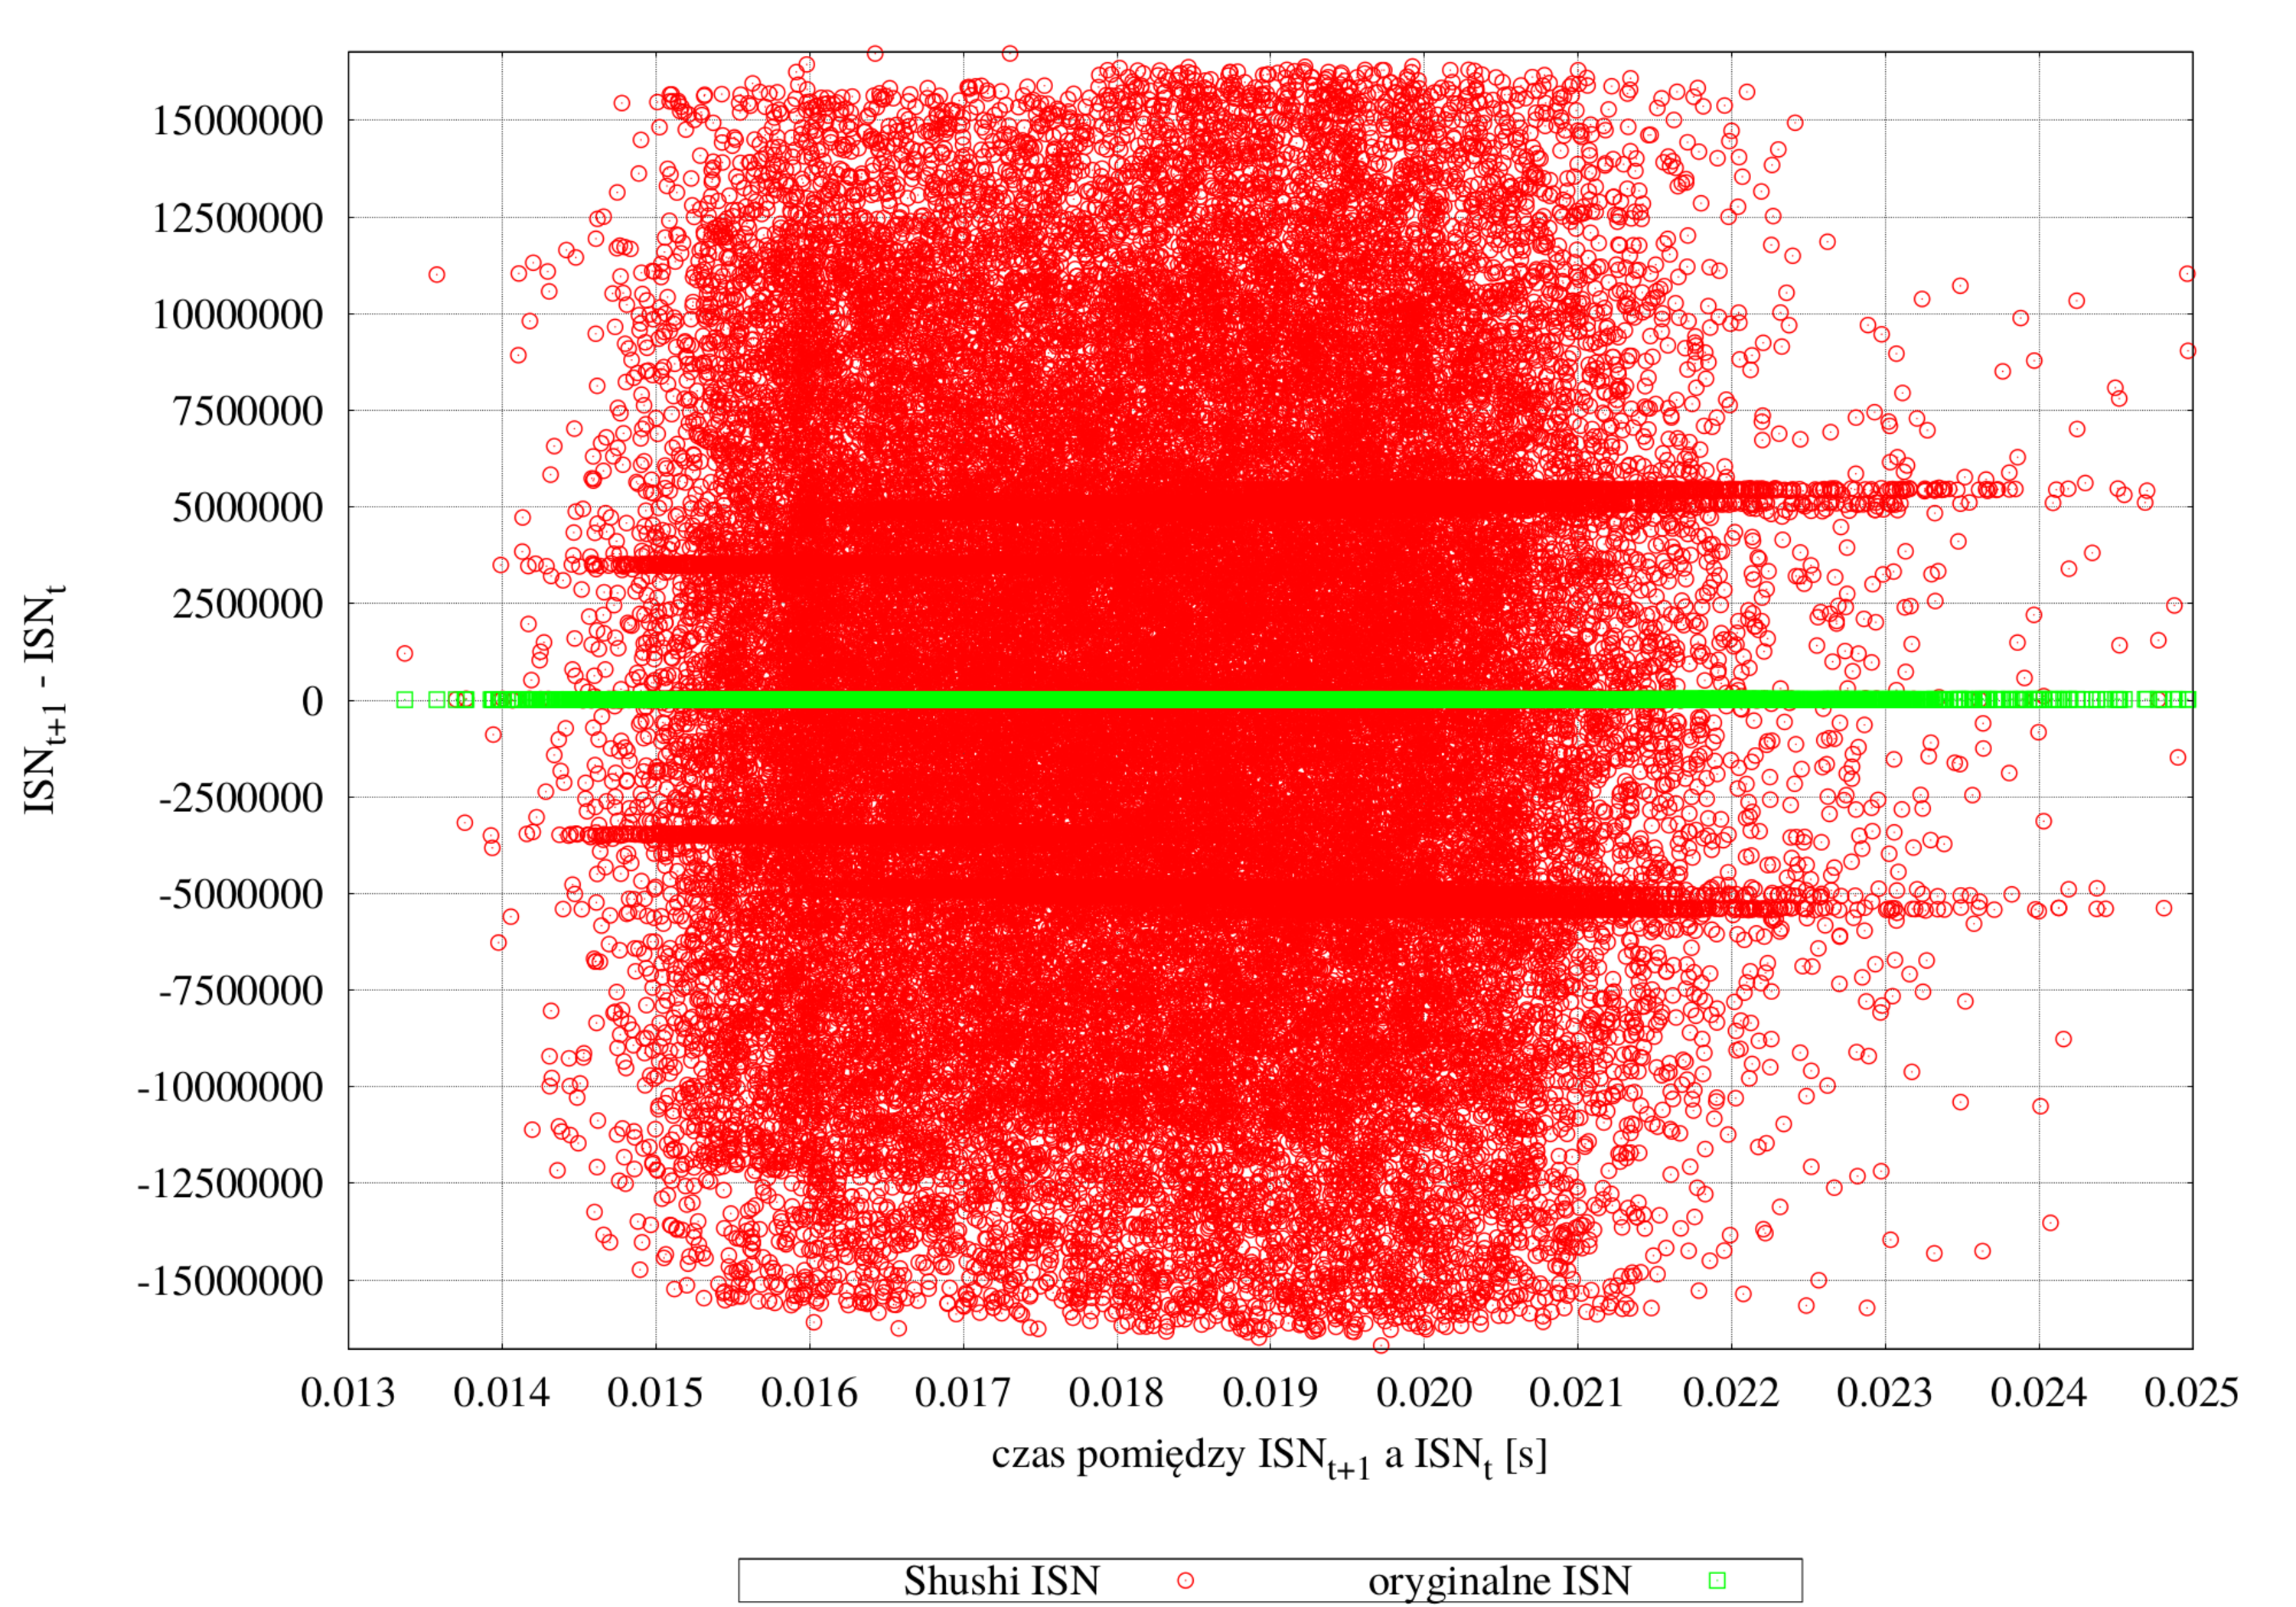
\includegraphics[scale=0.21]{\ImgPath/rys/IPPortRandDataDiff.pdf}
\end{center}
	\caption{Różnice pomiędzy kolejnymi numerami ISN wygenerowanymi przez 
jądro oraz \tech{Shushi}, stałe numery IP oraz porty TCP, losowe dane dla 
\tech{Shushi}, serie po około 60000 próbek.}
	\label{IPPortRandDataDiff}
\end{figure}
\fi

\begin{thebibliography}{99}
\addcontentsline{toc}{chapter}{Bibliografia}
\bibitem{gamejolt_page}{Gra Turbo Slam Dunk Unleashed w serwise GameJolt. \url{https://gamejolt.com/games/turbo-slam-dunk-unleashed/123485} [dostęp 14 stycznia 2019]}
\bibitem{unity_wiki} {Strona Wikipedi poświęcona Unity  \url{https://en.wikipedia.org/wiki/Unity_(game_engine)} [dostęp 17 stycznia 2019]}
\bibitem{canalplus_gry} {Twórcy Światów - Dokument zrealizowany przez Canal + \url{https://www.canalplus.pl/discovery/tworcy-swiatow}}
\bibitem{wiki_gameshistory} {Historia gier komputerowych na Wikipedi: \url{https://pl.wikipedia.org/wiki/Historia_gier_komputerowych} [dostęp 19 stycznia 2019]}
\bibitem{about_mono} {Oficjalna strona Mono \url{https://www.mono-project.com/docs/about-mono/} [dostęp 20 stycznia 2019]}

\end{thebibliography}

%\zakonczenie  % wklejenie recenzji i opinii

\end{document}
%+++ END +++
